\documentclass{article}

% \usepackage[position]{neurips_2026}

\usepackage[position,preprint]{neurips_2026}

% Remove the NeurIPS preprint notice from the first-page footnote.
\makeatletter
\renewcommand{\@noticestring}{}
\makeatother

\usepackage[utf8]{inputenc}
\usepackage[T1]{fontenc}
\usepackage{hyperref}
\hypersetup{colorlinks=true,linkcolor={blue!60!black},citecolor={blue!60!black},urlcolor={blue!60!black},anchorcolor=black,breaklinks=true}
\usepackage{url}
\usepackage{booktabs}
\usepackage{amsfonts}
\usepackage{nicefrac}
\usepackage{microtype}
\PassOptionsToPackage{table}{xcolor}
\usepackage{xcolor}
\usepackage{graphicx}
\usepackage{array}
\usepackage{tabularx}
\usepackage{enumitem}
\usepackage{tikz}
\usetikzlibrary{arrows.meta,positioning,shapes.geometric,fit,backgrounds}
\usepackage{placeins}
\usepackage{float}
\usepackage{multirow}

\title{From Scores to Knowledge Work: Rethinking AI Agent Evaluation}

\author{%
  Yining Hua$^{1}$\quad
  Hongbin Na$^{2}$\quad
  Cyrus Ayubcha$^{1}$ \quad
  Levi Lian$^{3,4}$\thanks{Corresponding author.} \\[0.4em]
  \small $^{1}$Harvard University \quad
  $^{2}$University of Technology Sydney \quad
  $^{3}$Stanford University \quad
  $^{4}$Raycaster AI \\[0.4em]
  \small \texttt{yininghua@g.harvard.edu} \quad
  \texttt{hongbin.na@student.uts.edu.au} \\
  \texttt{cyrusayubcha@hms.harvard.edu} \quad
  \texttt{levilian@raycaster.ai}
}

\begin{document}

\maketitle

\begin{abstract}
Knowledge work accounts for a large share of value in advanced economies and is a central target for current AI-agent deployment.
Agents are often evaluated as if high scores on public benchmarks establish readiness for drafting legal briefs, auditing financial records, running customer operations, or producing research memos.
Whether such inferences are warranted depends on what the benchmark actually measures and what claim its score is used to support.
\textbf{This position paper argues that knowledge-work capability should be evaluated on operations rather than isolated task fragments.}
We situate knowledge work and professional work in theories of non-routine judgment, jurisdiction, authority, and workflow-embedded artifacts. Based on the theories, we introduced two audit axes for benchmark claims.
\textit{Coverage} asks whether the benchmark targets the operation named in the claim, for which we develop an 18-operation taxonomy from 12{,}464 O{*}NET task statements.
\textit{Validity} asks whether the score supports the intended use of the output, separating task validity, including grounding, boundedness, and handoff, from organizational validity, including authority, accountability, and integration.
A detailed audit of \textsc{GDPval}, $\tau^2$-Bench, and \textsc{APEX-Agents} shows that these representative suites provide useful evidence about sampled deliverables, domain-specific episodes, and curated workspace tasks, but their scores remain narrower than general claims about knowledge-work or professional-work readiness.
We propose cross-occupation, stateful, rubric-graded evaluations centered on operations, together with clearer reporting guidelines for agent capability claims.
\end{abstract}

\section{Introduction}
\label{sec:intro}

Knowledge work, i.e., labor whose raw material and product are both knowledge and whose execution requires non-routine judgment \citep{drucker1959landmarks}, is the dominant share of value in advanced economies \citep{machlup1962production,porat1977information,drucker1999productivity}. It is the central target for AI-agent deployment across the professional, scientific, technical, financial, legal, educational, health-practitioner, and managerial portions of the labor market \citep{onet2024tasks,davenport2005thinking,grant1996kbv}. Substantial effort has gone into building agents for knowledge-intensive professional tasks.
Recent work has framed language-model agents as systems that can search, plan, use tools, maintain state, coordinate with users or other agents, and act over external work environments \citep{nakano2021webgpt,karpas2022mrkl,yao2023react,schick2023toolformer,park2023generative,wu2023autogen,wang2024survey}.

This attention reflects a broader expectation that agents will support the production of written artifacts, software changes, analyses, decisions, and other outputs central to knowledge work \citep{davenport2005thinking,brynjolfsson2026playbook,dellacqua2023jagged}.
Yet current AI-agent evaluation rarely treats knowledge work itself as the object under measurement: most evaluations score primitives such as retrieval, classification, reasoning, tool use, or patching, while the inferred capability claims name much richer activities such as legal analysis, financial audit, clinical administration, and research synthesis. 

The result of this evaluation practice is a structural mismatch between what evaluations score and what their scores are used to claim.
Recent enterprise-adoption surveys \citep{a16z2026adoption,brynjolfsson2026playbook} make the mismatch visible: adoption is concentrated in coding, the one area where agent evaluation has moved closest to operation-level work: coding benchmarks increasingly ask agents to modify real or repository-scale codebases in response to issue-like requests, with outputs judged through tests, patches, execution traces, or repository state changes \citep{jimenez2024swebench,kottamasu2026apex,swebenchpro2025}.
This makes coding evaluation closer to an operation-shaped setting than most other knowledge-work benchmarks, where stated capabilities often outrun deployment evidence, especially in regulated settings such as law, medicine, and audit \citep{kellogg2020algorithms,dellacqua2023jagged}.

We therefore take the position that 
\textbf{knowledge work should be evaluated on real work operations rather than isolated task fragments.} Primitive benchmark scores should not be cited as evidence of deployable knowledge-work capability unless the evaluation establishes both operation coverage and output validity.
Figure~\ref{fig:argmap} summarizes the audit structure that follows from this position.
We examine the problem by first defining knowledge work and then evaluating benchmark claims along two axes: \textit{coverage} and \textit{validity}.
Coverage asks whether the benchmark targets the operation named in the capability claim.
Validity asks whether the score supports the capability meaning attached to it; we separate \textit{task validity}, which concerns grounding, boundedness, and handoff, from \textit{organizational validity}, which concerns authority, accountability, and integration.

\begin{figure}[th]
\centering
\scriptsize
\begin{tikzpicture}[
  node distance=2.5mm and 6mm,
  every node/.style={font=\scriptsize, align=center},
  start/.style={draw, rounded corners=2pt, fill=gray!8, inner sep=3pt, text width=11.6cm},
  qbox/.style={draw, rounded corners=2pt, inner sep=3pt, text width=6.5cm},
  covq/.style={qbox, fill=orange!10, draw=orange!70!black},
  valq/.style={qbox, fill=teal!10, draw=teal!60!black},
  cov/.style={draw, fill=orange!6, draw=orange!70!black, rounded corners=2pt, inner sep=3pt, text width=6.5cm},
  val/.style={draw, fill=teal!6, draw=teal!60!black, rounded corners=2pt, inner sep=3pt, text width=6.5cm},
  endpt/.style={draw, rounded corners=2pt, fill=red!6, draw=red!60!black, inner sep=3pt, text width=13.4cm},
  arr/.style={-{Latex[length=1.8mm]}, semithick, gray!70!black},
]

\node[start] (kw) {\textbf{Knowledge work} \citep{drucker1959landmarks}: labor producing judgment-bearing outputs that move through review, approval, filing, and downstream use. The unit of evaluation is the \emph{operation} (\S\ref{sec:coverage-axis}), not the primitive or the occupation.};

\node[covq, below=5mm of kw, xshift=-3.7cm] (covq) {\textbf{Coverage} (\S\ref{sec:coverage-axis})\\Does the benchmark target the operation named in the claim?};

\node[valq, below=5mm of kw, xshift=3.7cm] (valq) {\textbf{Validity} (\S\ref{sec:validity-axis})\\Does the score support the intended use of the output?};

\node[cov, below=2.5mm of covq] (covlayer) {\textbf{Coverage evidence}: the benchmark must represent the work activity being claimed, not only a primitive such as retrieval, classification, reasoning, tool use, or patching.};

\node[val, below=3mm of valq, text width=3.1cm, xshift=-2cm] (vallayer_task) {\textbf{Task validity}\\Is the output a sound response to the assigned task?};

\node[val, below=3mm of valq, text width=3.1cm, xshift=2cm] (vallayer_org) {\textbf{Organizational validity}\\Can the receiving setting use the output?};

\node[cov, below=2.5mm of covlayer] (covlimit) {\textbf{Coverage limit}: a suite may score a primitive, a single-domain instantiation, or a small subset of professions while its score is read as evidence for deployable knowledge-work capability.};

% moved up by 0.5mm from 3mm to 2.5mm
\node[val, below=2.5mm of vallayer_task.south, xshift=1.7cm] (vallimit) {\textbf{Validity limit}: a score may reward fluent completion, format match, or local correctness while leaving grounding, boundedness, reviewability, and downstream usability untested.};

\node[endpt, below=3mm of covlimit.south, xshift=3.7cm] (end) {\textbf{Benchmark-to-knowledge-work overreach} (Section~\ref{sec:whybench}). Scores should be read at the level their evaluation design exercises, rather than as evidence of general knowledge-work or professional-work readiness.};

\draw[arr] (kw.south) -- ++(0,-2mm) -| (covq.north);
\draw[arr] (kw.south) -- ++(0,-2mm) -| (valq.north);

\draw[arr] (covq.south) -- (covlayer.north);
\draw[arr] (covlayer.south) -- (covlimit.north);

\draw[arr] (valq.south) -- ++(0,-1mm) -| (vallayer_task.north);
\draw[arr] (valq.south) -- ++(0,-1mm) -| (vallayer_org.north);

% vertical arrows to validity limit
\draw[arr] (vallayer_task.south) -- (vallayer_task.south |- vallimit.north);
\draw[arr] (vallayer_org.south) -- (vallayer_org.south |- vallimit.north);

% vertical arrows to final box
\draw[arr] (covlimit.south) -- (covlimit.south |- end.north);
\draw[arr] (vallimit.south) -- (vallimit.south |- end.north);

\end{tikzpicture}
\caption{Argument map. Two audit axes apply to claims that an AI agent is ready for knowledge work. Coverage asks whether the benchmark targets the operation named in the claim. Validity asks whether the score supports the intended use of the output. Coverage and validity limits together explain why benchmark scores are often read more broadly than their designs support.}
\label{fig:argmap}
\end{figure}
Together, coverage and validity limits explain benchmark-to-knowledge-work overreach: a suite may score a primitive, a single-domain instantiation, or a small subset of professions while its score is read as evidence for deployable knowledge-work capability. The rest of the paper develops this argument by distinguishing knowledge work from professional work (Section~\ref{sec:related}), building and cross-checking the 18-operation inventory (Section~\ref{sec:coverage-axis}), defining output validity (Section~\ref{sec:validity-axis}), and auditing \textsc{GDPval}, $\tau^2$-Bench, and \textsc{APEX-Agents} against both axes (Section~\ref{sec:whybench}).

\section{Knowledge Work}
\label{sec:related}
\textit{Knowledge work }is the canonical category of labor whose raw material and product are knowledge and whose execution requires non-routine judgment \citep{drucker1959landmarks}; it spans lawyers, physicians, accountants, financial analysts, management consultants, software engineers, data scientists, and many managerial and clerical roles. 
Typical outputs are judgment-bearing artifacts (e.g., contract clauses, diagnostic notes, audit findings, research memos, design specifications, regulatory filings, etc.) that move through review, approval, filing, and archival chains inside organizations \citep{suchman2007humanmachine,kellogg2020algorithms,barley1996technicians}.

Within knowledge work, \textit{professional work} is the strict subset whose practice is gated by legitimate jurisdiction over a problem domain, formal credentialing, industry-controlled entry, the authority to sign and file, and personal legal responsibility for the output \citep{abbott1988system,freidson2001professionalism}; lawyers admitted to the bar, licensed physicians, certified public accountants, and licensed professional engineers are paradigm cases.
Professional output is situated, distributed across review and authorization chains, and inseparable from the digital and non-digital infrastructure that algorithmic systems now enter and contest \citep{barley1996technicians,suchman2007humanmachine,kellogg2020algorithms}.

The literature often uses knowledge work and professional work interchangeably.
For evaluation, the key difference is that professional work carries an institutional layer, including credentialing, sign-off, and liability, that knowledge-work-content benchmarks do not exercise.
AI capability claims are often stated in professional-work language, such as ``can do legal analysis'' or ``can do clinical administration,'' yet supported by benchmarks that score domain content alone.
For example, \textsc{LegalBench}~\citep{legalbench2023} and \textsc{FinanceBench}~\citep{financebench2023} test tasks such as issue spotting and filings QA without evaluating credentialing, sign-off, or responsibility for use.
A per-literature discussion of how knowledge-work theory, professions sociology, IT economics, and the AI benchmark surveys frame the same cut is in Appendix~\ref{app:related}.

\section{Coverage and Validity in Knowledge Work Evaluation}
\label{sec:framework}

\subsection{Coverage of Operations}
\label{sec:coverage-axis}
\label{sec:realwork}
Coverage asks whether an evaluation targets the operation named in the attached capability claim.
An \emph{operation} is a recurring unit of knowledge work whose output is reviewed and used by downstream actors (i.e., the work activity being claimed, such as research synthesis, appraisal, administration, troubleshooting, or protocol execution).
A \emph{primitive} is a narrower model capability or task component (i.e., retrieval, classification, reasoning, tool use, or patching) that may support an operation but does not itself constitute one.
A primitive is therefore too small as the unit of coverage: retrieval alone does not establish research synthesis, classification alone does not establish appraisal, and tool use alone does not establish administration.
Nor is coverage established by benchmark size, domain realism, or task count if the scored unit remains a primitive or a narrow domain instance.

Our position does not reject primitive-level evaluation.
Primitive scores are useful for diagnosing component capabilities.
The problem is that current benchmark practice often treats primitives as proxies for operations even when the operation is only weakly represented: retrieval is read as research synthesis, classification as appraisal, tool use as administration, and patching as software engineering.
As Section~\ref{sec:whybench} shows, these proxies are often incomplete because they omit operation-level conditions such as grounding, scope control, judgment, handoff, and downstream use.

\subsubsection{Identifying Cross-Occupational Operations for Knowledge Work}
\label{sec:coverage-inventory}

Existing benchmark taxonomies do not define knowledge-work operations at the level needed to analyze whether evaluations cover cross-occupational work activities.
We therefore derive an 18-operation inventory from O{*}NET~30.2 occupation-specific task statements, using Job Zones~3--5 because they cover technical, professional, and managerial work \citep{onet2024tasks}.
O{*}NET is suited to this purpose because its task statements describe work activity rather than only occupations, skills, or worker attributes.
This task-level unit is also commonly used in studies that map AI capabilities to work \citep{eloundou2023gpts,felten2021occupational,webb2020aitasks}.

The starting corpus contains 12{,}464 O{*}NET task statements after filtering to Job Zones~3--5 and knowledge-work occupations.
We derive the inventory by screening out statements whose primary content is direct manual, performative, or routine clerical work, rewriting the retained statements into profession-neutral operation phrases, clustering them, and consolidating the resulting groups through expert-panel review.
The final inventory contains the 18 plain-English operations in Table~\ref{tab:ops}.
Each operation is defined by its input, output, adjacent-label contrasts, and cross-occupation examples spanning at least three occupation families.
For the operation counts in Table~\ref{tab:ops}, every statement in the 12{,}464-task corpus is assigned to one of the 18 final operation labels, so the reported counts conserve the screened corpus.
Construction details, sensitivity checks, and representative O{*}NET lines are in Appendices~\ref{app:taxonomy}, \ref{app:atlas-read}, and~\ref{app:mapping}.

The inventory maps knowledge-work activities, not professional authority.
O{*}NET task text does not encode credentialing, sign-off, liability, or responsibility for use.
Thus, operation coverage does not by itself establish professional-work readiness.

\label{sec:coverage-esco}
We use ESCO as an external legibility check rather than as a second derivation source \citep{esco2022v111}.
Holding the O{*}NET-derived inventory fixed, a rubric-based assignment of 5{,}826 scoped ESCO skill and competence items maps 5{,}730 items to one of the 18 operations ($98.3\%$), leaves 96 outside the inventory ($1.7\%$), and populates every operation.
This check supports the legibility of the operation labels outside O{*}NET, but it does not imply that O{*}NET and ESCO weight operations in the same way.
O{*}NET is a task-statement corpus, so it gives more weight to repeated work statements such as troubleshooting, administration, record keeping, investigation, appraisal, and teaching.
ESCO is a skill and competence catalogue, so it gives more weight to transferable competences such as advising, fabrication, coordination, design, and rule enforcement.
The full ESCO scope restrictions, non-mapped cases, and corpus-shift analysis are in Appendix~\ref{app:esco}.

\subsubsection{What the Operation Inventory Shows}\label{sec:coverage-shape}

Table~\ref{tab:ops} summarizes the 18 operations.
The counts report how often O{*}NET task statements are assigned to each operation; they do not measure economic value, deployment frequency, or the expected distribution of future AI-agent use.
The largest operations are \emph{analysis} (1{,}732), \emph{administration} (1{,}517), \emph{design} (992), \emph{inspection} (963), \emph{troubleshooting} (902), and \emph{record-keeping} (882), which together account for 6{,}988 of 12{,}464 assigned task statements ($56.1\%$).
This head of the distribution spans synthesis, organizational stewardship, specification, compliance checking, diagnosis, and canonical record production.

The middle and tail of the inventory are lower-frequency in O{*}NET task text, yet they remain central to knowledge work.
Operations such as \emph{advising}, \emph{appraisal}, \emph{investigation}, \emph{protocol-execution}, \emph{coordination}, \emph{representation}, \emph{emergency-response}, and \emph{rule-enforcement} often guide people, trigger procedures, allocate responsibility, or enter review and authorization chains \citep{abbott1988system,freidson2001professionalism,carlile2002pragmatic,malone1994coordination}.
For AI agents, these operations test capacities that standard retrieval and question-answering tasks only weakly expose: maintaining state over time, following a standard, stopping under uncertainty, preserving role boundaries, coordinating actors, escalating exceptions, and producing reviewable judgments \citep{suchman1987plans,weick2007managing,haynes2009surgical}.

Some operations already have partial decompositions into familiar primitives.
\emph{analysis} can involve retrieval, evidence selection, synthesis, and citation; \emph{record-keeping} can involve extraction, summarization, form filling, track of changes, and database update; \emph{appraisal} can involve classification or rubric scoring; and \emph{troubleshooting} can involve search, diagnosis, tool use, and repair \citep{lewis2020rag,petroni2021kilt,maynez2020faithfulness,ji2023hallucination,schick2023toolformer,yao2023react}.
Other operations still lack stable primitive decompositions.
\emph{coordination}, \emph{representation}, \emph{protocol-execution}, \emph{emergency-response}, and \emph{rule-enforcement} require state, timing, authority, exception handling, and responsibility assignment.
These requirements explain why operation-level evaluation needs more than the current primitive vocabulary.

\begin{table}[!ht]
\caption{The 18 cross-occupation operations derived from O{*}NET task statements.
Counts are assigned task statements, not labor-market weights or AI deployment estimates.
Full examples and adjacent-label contrasts are in Appendix~\ref{app:mapping}.}
\label{tab:ops}
\centering
\scriptsize
\setlength{\tabcolsep}{5pt}
\renewcommand{\arraystretch}{1.08}
\begin{tabular}{
@{}
>{\ttfamily\arraybackslash}m{0.23\linewidth}
>{\centering\arraybackslash}m{0.08\linewidth}
>{\raggedright\arraybackslash}m{0.62\linewidth}
@{}}
\toprule
\textbf{\normalfont Operation} & \textbf{\normalfont Tasks} & \textbf{\normalfont Definition} \\
\midrule
analysis & 1{,}732 & Synthesize evidence into a defended finding or interpretation. \\
administration & 1{,}517 & Plan, allocate, and steward organizational resources or processes. \\
design & 992 & Specify a system, plan, artifact, or service to satisfy a goal. \\
inspection & 963 & Check a present state against rules, standards, or specifications. \\
troubleshooting & 902 & Diagnose a problem and apply or recommend a remediation. \\
record-keeping & 882 & Create, update, store, and retrieve canonical organizational records. \\
teaching & 814 & Transfer knowledge or skill to a learner under review. \\
protocol-execution & 735 & Carry out a prescribed procedure with fidelity to the standard. \\
representation & 615 & Speak or act for an organization or client before others. \\
coordination & 603 & Align actors, constraints, dependencies, or timing around shared work. \\
creative-production & 543 & Produce an original creative or media artifact to a brief. \\
fabrication & 505 & Make, install, or maintain tangible assets under a work specification. \\
appraisal & 453 & Score, grade, or value an artifact or case against a standard. \\
advising & 403 & Tailor a recommendation to a specific person, client, or case. \\
investigation & 377 & Reconstruct an event, condition, or pattern from evidence. \\
emergency-response & 212 & Stabilize an acute incident under time pressure. \\
self-study & 186 & Maintain or update professional competency through learning. \\
rule-enforcement & 30 & Set, apply, or uphold behavioral or procedural rules in a setting. \\
\bottomrule
\end{tabular}
\end{table}

The inventory is occupation-agnostic by construction.
Each operation recurs across occupational lines, so the same operation can appear in multiple regions of the atlas when tasks share an activity pattern despite different professional vocabularies.
This is why each operation carries adjacent-label contrasts: verbs such as \emph{assess}, \emph{plan}, \emph{review}, and \emph{document} can point to different operations with different grading criteria.
The labels function as coverage units for benchmark audit, not as keywords.

\subsection{Validity}
\label{sec:validity-axis}

Coverage defines the qualitative scope of the audit: the operation tested, the setting in which it is tested, and the work relationships it represents.
Even with appropriate coverage, a benchmark can fail through rubric and scoring design: the score may reward fluent completion, format match, or local correctness while leaving grounding, boundedness, reviewability, and downstream usability untested.

Validity asks whether the scoring design measures the properties needed to support the benchmark's claim \citep{messick1989validity,Messick1995,aera2014standards,kane2013validating,jacobs2021measurement}.
In knowledge-work evaluation, the scored unit is usually an output artifact that later workflow steps receive: a brief, report, patch, filed record, recommendation, ticket, or decision note \citep{suchman1987plans,suchman2007humanmachine,carlile2002pragmatic,carlile2004transferring}.
A valid score must therefore be sensitive to the properties that make this artifact usable in the claimed setting.

Three features of knowledge-work outputs shape the required evidence:

\begin{enumerate}[label=(\roman*), leftmargin=*, nosep]
    \item The output draws on prior materials, such as records, policies, filings, source code, patient histories, financial statements, or previous decisions \citep{davenport2005thinking,carlile2002pragmatic,carlile2004transferring}.
    \item It is produced within an assigned role and scope, so some actions and conclusions are authorized while others are not \citep{drucker1967effective,simon1957admin,abbott1988system,freidson2001professionalism}.
    \item It is workflow-embedded: another person, team, system, or review step must be able to inspect it, rely on it, and act \citep{suchman1987plans,suchman2007humanmachine,carlile2002pragmatic,carlile2004transferring}.
\end{enumerate}

A score that ignores these elements may still measure local correctness, fluency, or tool completion, but it does not establish output validity for knowledge work.    


\subsubsection{Two layers of Validity.}\label{sec:two-layers}
We separate two layers of output validity.
\emph{Task validity} treats the output as a task artifact and asks whether it is a sound response to the assigned task.
It concerns grounding in the given materials, reasoning under the task constraints, and respect for assigned scope.
\emph{Organizational validity} treats the same output as a workflow action and asks whether the receiving setting can use it.
It concerns authority, accountability, sign-off, record integration, and compatibility with the next step \citep{bresnahan2002it,kellogg2020algorithms}. This distinction follows the measurement-theory separation between score meaning and score use \citep{messick1989validity,Messick1995,aera2014standards,kane2013validating} and the IT-economics point that technical capability often requires organizational complements before it produces workplace value \citep{bresnahan2002it}. A per-literature review of these precedents and recent field evidence is in Appendix~\ref{app:precedents}.

The two layers can fail independently.
An output may satisfy task validity while failing organizational validity.
For example, a draft memo may be grounded in the right sources, reasoned within the assigned question, and easy for a reviewer to inspect, yet still be unusable if no authorized actor can sign it, no accountable party owns the conclusion, or the workflow has no channel for accepting the artifact.
The reverse can also occur: an output may enter an organizational workflow while failing as a task artifact.

\emph{Mata v.\ Avianca} illustrates the task validity failure.
In this case, plaintiff's counsel opposed a motion to dismiss with legal authorities generated through ChatGPT \citep{mata2023avianca}.
The cited authorities appeared in a formal court filing and therefore entered litigation through attorneys who had authority to file on the client's behalf.
When opposing counsel and the court could not locate several cited decisions, counsel submitted purported copies or excerpts of the cases.
Those materials also contained non-existent opinions, false citations, and fabricated quotations.
The court sanctioned the attorneys and their firm under Rule 11, emphasizing that counsel had not verified the authorities before filing them.

\begin{table}[!ht]
\caption{Validity conditions for knowledge-work outputs.
Task validity concerns the assigned task; organizational validity concerns use in the receiving setting.}
\label{tab:validity}
\centering
\scriptsize
\setlength{\tabcolsep}{4pt}
\renewcommand{\arraystretch}{1.08}
\begin{tabularx}{\linewidth}{@{}m{0.18\linewidth} X@{}}
\toprule
\textbf{Condition} & \textbf{Question for Evaluation} \\
\midrule
\multicolumn{2}{@{}l}{\textbf{Task validity}} \\
\addlinespace[1pt]
Grounding
& Is the output supported by the governing materials, with correct source use, citation, and conflict handling? \\
Boundedness
& Does the output stay within the role, authority, and scope assigned by the task? \\
Handoff
& Can the next step parse, inspect, verify, and continue from the output? \\
\addlinespace[3pt]
\specialrule{0.35pt}{0pt}{1pt}
\multicolumn{2}{@{}l}{\textbf{Organizational validity}} \\
\addlinespace[1pt]
Authority
& Can the represented actor issue, accept, sign, file, or act on this output? \\
Accountability
& Is responsibility for using, reviewing, correcting, or rejecting the output locatable? \\
Integration
& Can the output enter the relevant record, system, review chain, or downstream workflow? \\
\bottomrule
\end{tabularx}
\end{table}

\paragraph{Task validity.}
Task validity decomposes into grounding, boundedness, and handoff. \emph{Grounding} requires a reliable relation between the output and the governing materials.
It fails when the output fabricates content, fabricates citations, ignores provided sources, uses a stale or non-governing source, or resolves conflicts without support \citep{maynez2020faithfulness,ji2023hallucination,lewis2020rag}.
Retrieval accuracy alone is insufficient because an output can retrieve the right document and still draw the wrong conclusion from it \citep{lewis2020rag,maynez2020faithfulness}. \emph{Boundedness} requires the output to stay within the role, authority, and scope assigned by the task.
It fails when the output makes an unauthorized conclusion, gives advice requiring a credential not represented in the task, changes a record it was only asked to summarize, or expands beyond the requested decision \citep{abbott1988system,freidson2001professionalism}. \emph{Handoff} requires the output to be usable by the next workflow step.
It fails when the recipient cannot parse the result, verify the evidence, locate the changed content, identify unresolved uncertainty, or integrate the output into the next action \citep{carlile2002pragmatic,carlile2004transferring,prov2013prov}.
Grounding, boundedness, and handoff do not substitute for one another: an output can be accurate but unauthorized, procedurally careful but unsupported, or locally correct but unusable by the next actor.

\paragraph{Organizational validity.}
Organizational validity concerns the receiving setting rather than the output alone.
It decomposes into authority, accountability, and integration.
\emph{Authority} asks whether the represented actor can issue, accept, sign, file, or act on the output.
It fails when the output requires a license, institutional role, approval right, or delegated authority that the task environment does not represent.
\emph{Accountability} asks whether responsibility for using, reviewing, correcting, or rejecting the output is locatable.
It fails when the output can affect downstream work without a responsible actor, reviewer, or correction path.
\emph{Integration} asks whether the output can enter the relevant record, system, review chain, or downstream workflow.
It fails when the output is locally correct but cannot be filed, versioned, reconciled with existing records, or acted on by the next system or person.

Many benchmarks can test output-side handoff, such as format, provenance, or reviewability.
Fewer test organizational handoff, where the output must be accepted by a role-bearing actor or enter a record of practice.
This distinction limits the claim attached to the score: output-side handoff supports stronger task-validity evidence, while authority, accountability, and integration are needed before the score can support professional-work readiness.

\subsubsection{What the Validity Conditions Show}
\label{sec:validity-patterns}

Some current evaluations and benchmarks reflect parts of this validity structure.
Grounding is most visible when a benchmark supplies source files, policies, records, spreadsheets, webpages, or other governing materials and scores whether the output uses them correctly.
Boundedness is most visible when the task defines an actor, an instruction scope, available tools, forbidden actions, or policy constraints.
Handoff is most visible when the scored output is not only an answer, but a patch, edited document, spreadsheet, filled form, browser state, ticket update, or other artifact that another actor could inspect.

These conditions map unevenly onto existing evaluation formats.
Coding benchmarks provide the strongest task-validity evidence because repository state, issue specifications, patches, and tests make the handoff object executable and checkable \citep{jimenez2024swebench,deng2025swebenchpro}.
Data-analysis and data-science benchmarks make analytic work partly inspectable when agents operate over data files, execution environments, closed-form answers, or modeling tasks.
Their verifiers, however, usually cover only the parts of analysis that fit the benchmark's output format \citep{hu2024infiagent,jing2024dsbench}.
Document, retrieval, and office benchmarks strengthen grounding by giving the model source documents, tables, emails, calendars, policies, or enterprise corpora.
They often still score a final answer or task state rather than a reviewable work product \citep{opsahlong2026officeqapro,wang2024officebench}.

Spreadsheet and table-work benchmarks can check values, formulas, joins, workbook structure, and robustness across test cases, while assumptions, audit trails, linked-object effects, and later reuse often remain implicit \citep{ma2024spreadsheetbench}.
Web, computer-use, and enterprise-workflow benchmarks test bounded action through applications, tools, websites, enterprise systems, users, and world state, yet often stop once the local target state is reached \citep{zhou2023webarena,drouin2024workarena,boisvert2024workarenaplus,xie2024osworld}.
Dialogue and customer-support benchmarks make policy following, interaction quality, shared-state tracking, and user coordination more visible, while post-interaction records, escalation, correction, and responsibility are usually weaker \citep{barres2025tau2}.
Legal, financial, and professional-deliverable benchmarks improve domain or face validity by asking for legal reasoning, financial question answering, occupational deliverables, or client-like professional-service outputs.
In these settings, answer correctness, expert preference, or rubric satisfaction can collapse grounding, boundedness, handoff, and domain judgment into one quality signal \citep{guha2023legalbench,islam2023financebench,gdpval2025,vidgen2026apexagents}.

The organizational layer is less often evaluated.
Authority requires the benchmark to represent who may issue, approve, file, or act on the output.
Accountability requires a responsible reviewer, owner, or correction path.
Integration requires the output to enter a durable record, workflow state, review queue, or downstream system.
Most current benchmarks represent files, tools, and task state more often than they represent authority, responsibility, and workflow uptake.
As a result, their scores usually support task-validity claims before they support organizational-validity claims.

The general pattern is that benchmarks become more valid for knowledge work when they expose more of the work object to scoring: sources, code, data, artifacts, tools, state, policies, interaction history, and downstream records.


\section{What Current Benchmarks Measure}
\label{sec:whybench}

Coverage and validity determine how benchmark scores should be read.
We audit three representative suites that foreground realistic agents or deliverables: \textsc{GDPval}~\citep{gdpval2025}, $\tau^2$-Bench~\citep{barres2025tau2}, and \textsc{APEX-Agents}~\citep{vidgen2026apexagents}.
These suites are the benchmarks frontier model releases most prominently cite under their knowledge-work or professional-capability sections, and they span the three argumentative shapes vendors use to justify a knowledge-work readiness claim: expert-graded deliverable (\textsc{GDPval}), stateful interaction ($\tau^2$-Bench), and curated professional workspace (\textsc{APEX-Agents}).
For each suite we read the released task prompts, reference files, and rubric items against the two audit axes; per-task counts in this section are computed from the released task and rubric files, and a consolidated scorecard with per-suite case material is in Appendix~\ref{app:benchcases} (Table~\ref{tab:audit-three}).
The aim is claim interpretation rather than benchmark ranking.
A wider audit covering 30 additional public benchmarks is in Appendix~\ref{app:audit-table}, the per-benchmark coverage reasoning behind that audit is in Appendix~\ref{app:perbench}, and the recurring failure surfaces these benchmarks share are catalogued in Appendix~\ref{app:surfaces}.
The unit of analysis underlying the audit, the three-profession threshold for cross-occupation evidence, and the structural features a benchmark must preserve to score the operation rather than a primitive inside it, are set out in Appendix~\ref{app:unit-features}.

\textbf{\textsc{GDPval}} releases 220 tasks across 44 occupations sampled in nine sectors (Professional, Scientific and Technical Services; Government; Information; Manufacturing; Real Estate; Finance and Insurance; Wholesale Trade; Health Care; Retail), with five tasks per occupation in the public release.
Each task supplies a prompt, a set of reference files, and an expected deliverable shape such as a document, presentation, diagram, spreadsheet, or multimedia file.
Grading is rubric-driven: the release contains 10{,}453 human-authored criterion items distributed across the 220 tasks (mean 47.5 per task; range 14--137), each carrying a numeric score (mostly $+1$ or $+2$, with explicit penalty items at $-10$ and $-20$ for output-fidelity violations such as lossy audio compression or sounds absent from the reference set).
Criterion items fall into four kinds: mechanical format checks (501 items), substantive correctness statements (871), institutional fidelity to reference materials (693), and other content-presence checks (8{,}388 items).

\textit{Coverage.}
The primitives the benchmark scores are content extraction from supplied reference files, document and spreadsheet assembly under named formats, fact-presence and named-correctness checking against domain references, and adherence to delivery-format constraints.
The operations these primitives instantiate vary with the deliverable: a task may bundle \emph{analysis}, \emph{design}, \emph{record-keeping}, \emph{advising}, and at times \emph{creative-production} or \emph{inspection}, while the unit of measurement is artifact production rather than the operation itself.
The judgment-in-acquisition phase of the named operation, where a practitioner negotiates source completeness, scopes the engagement, or validates the population against a system of record, is performed by the prompt designer rather than by the agent.
Of the 220 tasks, 95 (43.2\%) supply no reference files at all; the median per-task reference-file count is 1, and 191 of 220 tasks (86.8\%) supply at most two reference files.
Tasks for Lawyers, Software Developers, Concierges, and First-Line Supervisors of Police and Detectives supply zero reference files in all five tasks; Nurse Practitioners, Personal Financial Advisors, Financial and Investment Analysts, and General and Operations Managers each supply zero reference files in four of five.
Cross-occupation breadth is wide (44 occupations); per-occupation depth is shallow (five tasks); per-operation evidence is therefore dispersed across the corpus rather than concentrated within any single operation cell.

\textit{Validity.}
Task-validity evidence is concentrated on artifact form rather than on the analytic operation the occupational label names.
Roughly 91\% of rubric items reward artifact form rather than analytic depth: file-format compliance (mechanical, 4.8\% of items), verbatim source-fidelity (institutional, 6.6\%), and expert-written per-task content strings (other, 80.2\%); the remaining 8.3\% of items (substantive) carry named-formula or named-correctness statements.
Grounding is partly visible on the 56.8\% of tasks that supply at least one reference file through institutional items (e.g., copying source rows verbatim, preserving audio fidelity), while substantive items are closed-form: each criterion encodes a single pre-specified correct answer rather than admitting the range of defensible answers a real analysis tolerates.
Boundedness is implicit: the rubric assumes the represented role rather than penalizing scope creep or out-of-role advice.
Handoff is not scored because the rubric does not check whether the deliverable would be accepted by an authorized reviewer, signed, filed, or carried into a downstream record.
Organizational validity is not tested: authority, accountability, and integration into an organizational queue are absent from the criterion set.
The score supports artifact-production fidelity and named-correctness recall under occupational labels; analytic operation depth, judgment under defensible-answer ambiguity, and cross-occupation operation coverage require further evidence.

\textbf{$\tau^2$-Bench} evaluates conversational agents over four customer-service domains: telecom (2{,}285 episodes), retail (114), banking-knowledge (97), and airline (50), totaling 2{,}546 episodes with telecom dominant by an order of magnitude.
The agent and a simulated user share access to a stateful world.
Success is reduced to a Boolean reward by programmatic checks expressed against the action trace, the environment assertion, the database state, a substring or fact match against the user-facing message, or a communicate predicate.

\textit{Coverage.}
The primitives the benchmark scores are tool calls under a fixed API, dialogue management with a simulated user, state tracking against a programmatic world, and policy-conditioned instruction following.
The operations these primitives instantiate are partial \emph{administration}, \emph{coordination}, and at times \emph{troubleshooting}, exercised as customer-service episodes within four service stacks.
Customer-service occupations are classified in O{*}NET Job Zone~2 (vocational preparation), while the audit framework in Section~\ref{sec:related} anchors knowledge work in Job Zones 3--5; episodes graded in $\tau^2$-Bench therefore exercise an interaction and policy-compliance work shape distinct from the analytic operations the framework targets~\citep{onet2024tasks}.
Cross-domain claims grounded in $\tau^2$-Bench are in practice claims about telecom episodes, since the telecom split contains 2{,}285 of 2{,}546 episodes (89.7\%).

\textit{Validity.}
Task-validity evidence is the strongest of the three suites: policy, tools, and world state make grounding and permitted action visible, and a fixed action and assertion vocabulary makes boundedness checkable.
The simulated user is pre-loaded with the problem statement, persona, persistence behavior, and acceptance criteria; for example, a roaming-customer telecom episode scripts the user's brief to ``\emph{you absolutely want to get excellent internet speed on your phone~\ldots~you will not consider the issue resolved until speed test returns excellent internet speed},'' so the interpretive step where competent customer-service work distinguishes itself (clarifying what the customer is asking) is performed by the simulator rather than by the agent.
The user-facing message and communicate checks provide a within-episode handoff test because the agent must convey information to the simulated user before the episode ends, and no record persists past episode termination: the simulator does not represent a ticket queue, an account-note system, an escalation owner, or a downstream filing path.
Organizational validity is not tested: durable record entry, downstream review, assigned responsibility, escalation ownership, and integration into an organizational queue go unscored.
The score supports policy-compliant coordination of customer-service episodes against scripted users in the represented domains; broader customer-service competence and knowledge-work readiness require further evidence.

\textbf{\textsc{APEX-Agents}} matches the framework's working definition of knowledge work more closely than any other public benchmark currently in release: 480 tasks evenly distributed across investment banking, management consulting, and corporate law (160 per domain), staged over 33 expert-curated worlds (10 banking, 11 consulting, 12 law) that contain on average 166 files including documents, spreadsheets, PDFs, email, chat, calendar, presentations, and a code-execution surface, with web search disabled.
The body of the analysis below should be read as identifying structural limits at the closest current substrate, rather than defects peculiar to this suite.
The supporting workspace is constructed for the benchmark: experts in role produce the engagement record from scratch over multi-week sessions, sending emails, drafting memos, scheduling meetings, and iterating on spreadsheets and slide decks, so the file system the agent navigates is authored content rather than the residue of an actual engagement~\citep{vidgen2026apexagents}.
Of the 33 worlds, 22 use entirely fictional entities, 9 place real companies in fictional scenarios, and 2 mix real and fictional companies, and the engagements are therefore roleplay without a real partner, client, filing path, or downstream consumer of the agent's output.
Each task is graded against a short list of binary criteria (mean 4.06; range 1--10), each phrased as a positive statement the response must satisfy (e.g., ``States that the force majeure clause can be invoked for tariff increases of more than 25\%'').

\textit{Coverage.}
The primitives the benchmark scores are long-context retrieval over a file-rich workspace, fact extraction across heterogeneous file formats, and the drafting of a short response or, less often, a structured artifact.
Output formats are skewed: 422 of 480 tasks (87.9\%) expect an inline reply, while only 58 tasks (12.1\%) require an artifact (document, spreadsheet, or slide deck) to be created or edited inside the world; the dominant scored unit is a short message judged against three to five fact-presence criteria.
Operations whose output is structurally an artifact rather than a message (\emph{record-keeping}, \emph{protocol-execution}, \emph{appraisal}, \emph{creative-production}) fall outside the reply-only majority by output shape.
Task prompts also pre-supply the analytical scaffolding of the named operation: a representative consulting task fixes the analytical assumptions inline (``\emph{West North Central division plant locations only have a 10\% annual efficiency gain from labor cost. For other locations, the efficiency gain is 20\%. However, the efficiency gain is 5\% for non-unionized production supervisors no matter where they are located}''); a law task asserts the case theory as fact (``\emph{this was all documented in email exchanges and in meetings with Ava's counsel}''); an investment-banking task supplies the model itself (``\emph{from the figures in merger model, please recalculate the stock portion of the offering price}'').
The operations these primitives instantiate are mostly \emph{analysis} and \emph{advising} executed against pre-supplied premises, with some \emph{design}, \emph{coordination}, and \emph{record-keeping} where artifact outputs are required, concentrated in three professional-services settings.

\textit{Validity.}
Task-validity evidence is stronger than in answer-only benchmarks because in-world files, disabled web search, structured prompts, output-format flags, and rubric criteria make grounding, boundedness, and partial handoff visible.
Grounding holds for the operative document the prompt names, with the caveat that the surrounding workspace the agent interrogates is authored content produced for the benchmark rather than residue from a real engagement, so signals an analyst would weigh in practice (a vendor's irregular email cadence, a CC list that betrays a side conversation, a typo a partner would notice) are absent by construction.
The rubric vocabulary does not reward the professional move of interrogating the supplied premises: a clarification response (``I would need to verify which amendment governs before confirming whether tariff increases of that magnitude are covered'') fails the binary criterion that requires the response to ``state that the force majeure clause can be invoked for tariff increases of more than 25\%.''
Handoff is partially scored on the 12\% of tasks that produce an artifact; the 87.9\% inline-reply majority terminates at a short message even when the world supplies the artifactual surface (Word, Excel, Powerpoint applications populated with engagement-relevant content) on which a partner could review the work.
Organizational validity is not tested: the rubric checks whether stated facts appear in the response, the worlds are roleplay engagements without a real partner, client, filing path, or downstream consumer, and whether the response can be signed, filed, relied on by a partner or client, accepted into a formal record, or made accountable inside an actual engagement is unscored.
The score supports analysis and advising on pre-supplied premises in curated professional-services worlds, scored at the chat surface; cross-occupation operation coverage, premise interrogation, artifact handoff, and organizational integration require further evidence.

\paragraph{Roll-up.}\label{sec:rollup}
The shared pattern is claim limitation at the upstream end of each operation.
Each suite scores the post-judgment fragment of the work it labels.
\textsc{GDPval} reaches the agent only after sources have been gathered, scoped, and validated by the prompt designer; 43.2\% of tasks supply no source files at all.
In $\tau^2$-Bench, the simulated user arrives pre-loaded with the problem, the persona, and the acceptance criteria, leaving execution rather than interpretation as the agent's task.
\textsc{APEX-Agents} grades chat replies inside roleplay engagements whose supporting workspace is authored for the benchmark and whose analytical premises are supplied in the prompt.
Each suite makes important parts of knowledge work observable.
None establishes cross-occupation operation coverage, judgment-in-acquisition, premise interrogation, artifact handoff, or organizational integration.
Benchmark scores should therefore be read at the level their design exercises, rather than as evidence of general knowledge-work or professional-work capability.
\section{Alternative views}
\label{sec:altviews}
A first alternative view is that realistic tasks and expert-graded deliverables are sufficient for evaluating knowledge work.
On this view, if a benchmark uses real work products, domain experts, source files, and plausible outputs, it already captures the relevant capability.
Our concern is that realism alone does not fix the score's inferential scope.
A task may resemble professional work while still scoring a one-shot deliverable, a single-domain episode, or a local artifact state.
Such scores can provide useful evidence about task performance, but they do not establish cross-occupation operation coverage or organizational validity unless the design also represents the operation, the handoff object, and the receiving workflow.

A second alternative view is that the gap between benchmark progress and workplace adoption reflects security, data access, integration, governance, and change management rather than evaluation.
These factors are real.
They also define part of what deployment-relevant evaluation must make explicit.
A benchmark that does not represent permission boundaries, review handoff, durable state change, or receiving-system constraints cannot distinguish remaining deployment friction from unsupported capability claims.
Evaluation is therefore part of deployment reasoning because it fixes the scope of what a benchmark score can be used to claim.

A third alternative view is that operation-level evaluation is too costly.
Cross-occupation tasks, stateful environments, and expert review are expensive.
The response is to keep primitive benchmarks for diagnosis while building reusable verifier infrastructure for stronger claims.
Simulators, rubric lanes, failure-mode taxonomies, and public work corpora are what make operation-level evaluation repeatable.
Code-review benchmarks show that an operation becomes more tractable once a corpus, artifact format, and checkable verifier exist \citep{sweprbench2025,codefusecrbench2025,withmartiancr2024}.
Similar verifier paths are still needed for analysis, administration, appraisal, and other knowledge-work operations.
Detailed responses are in Appendix~\ref{app:altviews}.

\section{Future directions}
\label{sec:future}

Future work should first strengthen the operation inventory.
O{*}NET provides broad occupation-linked task statements, but it is still an occupational database: its task text aggregates across workplaces, updates unevenly, and gives limited evidence about local workflow, authority, and responsibility \citep{handel2016onet}.
Operation taxonomies should be checked against workflow traces, expert protocols, professional standards, case files, enterprise tickets, and cross-national occupational taxonomies.
The goal is a better account of the work operation named in an evaluation claim.

A second direction is to map examinable primitives to operations.
Retrieval, classification, tool use, code execution, source attribution, editing, and state tracking should be located inside the work operation they support.
For example, \emph{appraisal} may combine evidence retrieval, rubric application, comparative judgment, and an auditable finding.
\emph{record-keeping} may combine extraction, normalization, provenance preservation, and update of a canonical record.
\emph{protocol-execution} may combine state tracking, ordered actions, exception handling, and escalation.
This would make it clearer whether a benchmark evaluates a primitive, an operation component, or an operation.
A per-operation translation to AI-task formulations and the principal open scoring problem standing between naming an operation and measuring it is summarized in Appendix~\ref{app:opslens}.

A third direction is scoring design.
Knowledge-work benchmarks should state which validity conditions their scoring rules test.
Automatic checks can cover some signals, including tests, state diffs, formula checks, source matching, and schema validation.
Other signals require expert rubrics, provenance review, counterfactual cases, or downstream continuation tasks.
Scores should keep these signals separable when possible, so that benchmark results can distinguish unsupported evidence, scope violation, poor handoff, and failed workflow uptake.

Finally, conferences, journals, benchmark papers, and model reports should adopt guidelines for reporting agent capabilities.
Submissions and technical reports should state the scored unit, the represented operation, the occupation or domain scope, the validity conditions tested, and the highest claim supported by the evaluation design.
They should also mark unsupported extrapolations, such as using answer accuracy, tool success, or deliverable preference as evidence of professional or organizational readiness.
This would make overclaiming easier to identify at review time and make benchmark results easier to interpret after publication.

\section{Conclusion}
\label{sec:conclusion}

This position argued that knowledge-work capability should be evaluated at the level of operations: recurring units of work whose outputs are reviewed, continued, and acted on downstream.
It introduced two audit axes for reading benchmark claims.
Coverage asks whether the benchmark targets the operation named in the claim.
Validity asks whether the score supports the intended use of the output, separating task validity from organizational validity. The O{*}NET-derived operation inventory and ESCO check provide a starting point for coverage analysis.
The benchmark audit shows that current suites can make parts of knowledge work observable, but their scores often remain narrower than claims about general knowledge-work or professional-work readiness.
Future evaluations should report the scored unit, represented operation, domain scope, validity conditions tested, and highest claim supported by the design.

{\small
\bibliographystyle{plainnat}
\bibliography{references}
}

\newpage
\appendix
\renewcommand{\thefigure}{\Alph{section}.\arabic{figure}}
\renewcommand{\thetable}{\Alph{section}.\arabic{table}}
\makeatletter
\@addtoreset{figure}{section}
\@addtoreset{table}{section}
\makeatother
\setcounter{figure}{0}
\setcounter{table}{0}

\section{Extended related work}
\label{app:related}

This appendix expands Section~\ref{sec:related} with the literatures that bear on the audit framework but were summarised only briefly in the main text.

\paragraph{Economics of AI and task-level exposure.} A productive strand estimates the extent to which current AI capabilities bear on occupations by mapping tasks to capability vectors.
Patent text supplies one input \citep{webb2020aitasks}, rubric-matched capabilities feed the AI Occupational Exposure index from O{*}NET abilities \citep{felten2021occupational}, expert-rubric procedures over task descriptions formalise suitability for AI-related automation \citep{brynjolfsson2018sml}, and the same procedure has been applied at LLM scale \citep{eloundou2023gpts}.
Benchmarks and cognitive abilities are bridged explicitly \citep{tolan2021baioe}, and a running capability tracker compiles results across suites \citep{epoch2024capability}.
These efforts deliberately avoid the public-benchmark layer when making claims about real work, anchoring instead on O{*}NET tasks combined with rubric procedures.
We read this design choice as implicit evidence that researchers in those traditions do not treat the benchmark layer as sufficient for the claim; our audit gives a constructive account of \emph{why}.

\paragraph{AI benchmark surveys and task taxonomies.} Prior taxonomic work has largely organised benchmarks by \emph{primitive} (question-answering, summarisation, code synthesis, multiple choice, tool use) rather than by operation.
Surveys of agent benchmarks \citep{webarena2023,workarena2024,osworld2024,officebench2024,gaia2023} systematically widen the environment while keeping the scoring unit short (atomic success, exact match, reward).
Industry reports framing AI in terms of cognitive automation and agentic deployment \citep{a16z2026adoption,brynjolfsson2026playbook,microsoft2024workplaces} similarly aggregate primitive scores when reasoning about work-readiness.
Position-style critiques have flagged that the evaluation instrument and the model jointly produce adoption friction; our work is complementary in that we critique the unit of scoring rather than the evaluator architecture.
Within code, the lineage \textsc{HumanEval}~\citep{chen2021humaneval}~$\to$~\textsc{SWE-bench}~\citep{jimenez2024swebench}~$\to$~\textsc{APEX-SWE}~\citep{kottamasu2026apex} and \textsc{SWE-bench Pro}~\citep{swebenchpro2025} shows that operation-shaped evaluation is feasible where execution verifiers exist, and recent code-review benchmarks \citep{sweprbench2025,codefusecrbench2025,withmartiancr2024} are early existence proofs that the appraisal operation is also scoreable.

\section{Taxonomy construction details}
\label{app:taxonomy}

This appendix documents how the 18-operation taxonomy is built from O{*}NET task text.
Figure~\ref{fig:pipeline} diagrams the full pipeline, including the embedding and HDBSCAN clustering stage that yields 108 dense task groups before expert-panel consolidation.

\paragraph{Corpus.} O{*}NET 30.2 task statements, filtered to Job Zones 3--5 and knowledge-work occupations: 12{,}464 tasks retained of 12{,}611 (99\%; 147 dropped).
Each row carries the O*NET-SOC code, occupation title, task identifier, cleaned task text, importance and relevance scores, and Job Zone.

\paragraph{Screens.} A knowledge-work prescreen removes direct-embodied tasks (pass~0) and yields the 12{,}464-task corpus.
The task-level screen categories are developed by three independent 100-task samples drawn without replacement from this 12{,}464-item corpus; each sample is adjudicated against a growing list of candidate exclusion categories until the category list stabilises at twelve (direct-manual, performative, routine-clerical, and their sub-variants).
The stabilised screen is then applied to the full corpus, removing 4{,}092 tasks and retaining 8{,}372 tasks (including a 34-task audit re-inclusion from an availability-scheduling cluster) on which all subsequent embedding, clustering, and consolidation is performed.

\paragraph{Embedding and clustering.} Tasks are rewritten into profession-neutral operation phrases under a fixed prompt to remove domain vocabulary, then embedded into a $1{,}536$-dimensional space and $L_{2}$-normalized.
UMAP (15 dimensions, 30 neighbors, cosine metric) followed by HDBSCAN (minimum cluster size 30, minimum samples 10, excess-of-mass extraction) yields 108 clusters on the task-only geometry; noise is soft-assigned via membership vectors.

\paragraph{Consolidation.} Four rounds of LLM summarisation interleaved with expert-panel review produce a domain-stripped sub-operation label per cluster and a top-level operation set.
Rounds 1--3 produced 38, 39, and 16 top-level operations respectively and were rejected by the panel; round 4 produced the 18 plain-English, single-concept operations used in Figures~\ref{fig:pipeline} and~\ref{fig:atlas} and Table~\ref{tab:ops}, including the split of an earlier compliance-audit operation into \emph{inspection} and \emph{investigation} and the folding of a small clinical~/~surgical~/~nursing-support cluster (93 tasks) into \emph{protocol-execution}.

\paragraph{Invariants.} Every cluster has exactly one top-level assignment; all 12{,}464 tasks are conserved across assignment; every top-level operation has $\geq\!1$ member cluster and $\geq\!3$ distinct profession families in its cross-occupation example set; every operation carries an explicit set of contrasts against every adjacent operation.

\begin{figure}[!htbp]
\centering
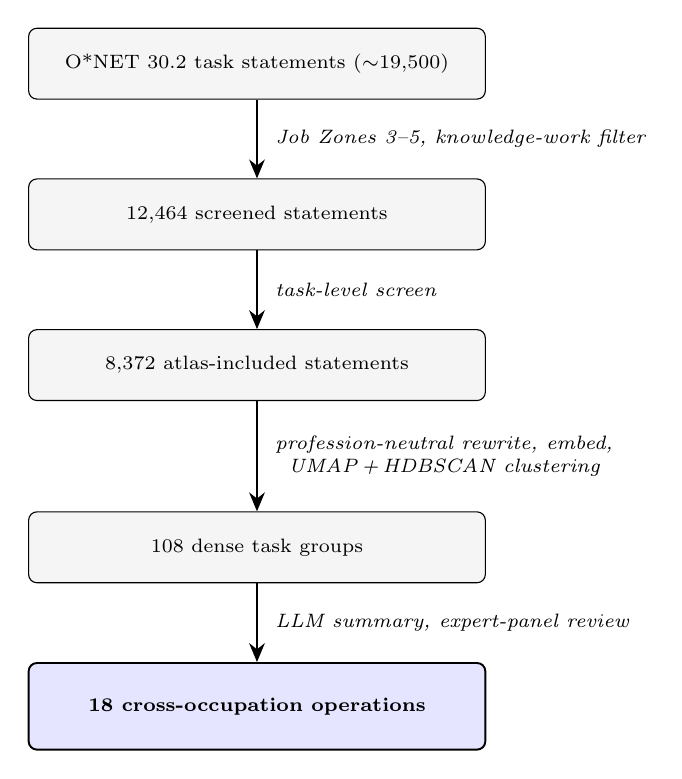
\begin{tikzpicture}[
  font=\scriptsize,
  every node/.style={align=center},
  data/.style={
    draw, rounded corners=3pt, fill=gray!8,
    inner sep=5pt, minimum height=9mm, minimum width=58mm,
    line width=0.4pt
  },
  final/.style={
    draw, rounded corners=3pt, fill=blue!10,
    inner sep=5pt, minimum height=11mm, minimum width=58mm,
    line width=0.7pt, font=\scriptsize\bfseries
  },
  arr/.style={-{Stealth[length=2.4mm,width=2mm]}, line width=0.55pt},
  lbl/.style={right=3pt, font=\scriptsize\itshape, anchor=west}
]
\node[data] (raw) {O{*}NET~30.2 task statements ($\sim$19{,}500)};
\node[data, below=10mm of raw] (screened) {12{,}464 screened statements};
\node[data, below=10mm of screened] (retained) {8{,}372 atlas-included statements};
\node[data, below=14mm of retained] (groups) {108 dense task groups};
\node[final, below=10mm of groups] (ops) {18 cross-occupation operations};

\draw[arr] (raw) -- node[lbl]{Job Zones 3--5, knowledge-work filter} (screened);
\draw[arr] (screened) -- node[lbl]{task-level screen} (retained);
\draw[arr] (retained) -- node[lbl]{profession-neutral rewrite, embed,\\UMAP\,+\,HDBSCAN clustering} (groups);
\draw[arr] (groups) -- node[lbl]{LLM summary, expert-panel review} (ops);

\end{tikzpicture}
\caption{Construction pipeline for the 18-operation inventory.
O{*}NET~30.2 task statements are filtered to Job Zones~3--5 and knowledge-work occupations, leaving 12{,}464 task statements.
A stricter task-level screen retains 8{,}372 statements for profession-neutral rewriting, embedding, and HDBSCAN clustering on a UMAP projection, which yields 108 dense task groups.
Four rounds of LLM summarization and expert-panel review consolidate the groups into 18 cross-occupation operations.
For Table~\ref{tab:ops}, the final 18 operation labels are applied back to the full 12{,}464-task screened corpus, so the per-operation counts conserve the screened corpus rather than the 8{,}372-task atlas-included subset.}
\label{fig:pipeline}
\end{figure}
\FloatBarrier

\section{Reading the operation atlas}
\label{app:atlas-read}

\begin{figure}[t]
\centering
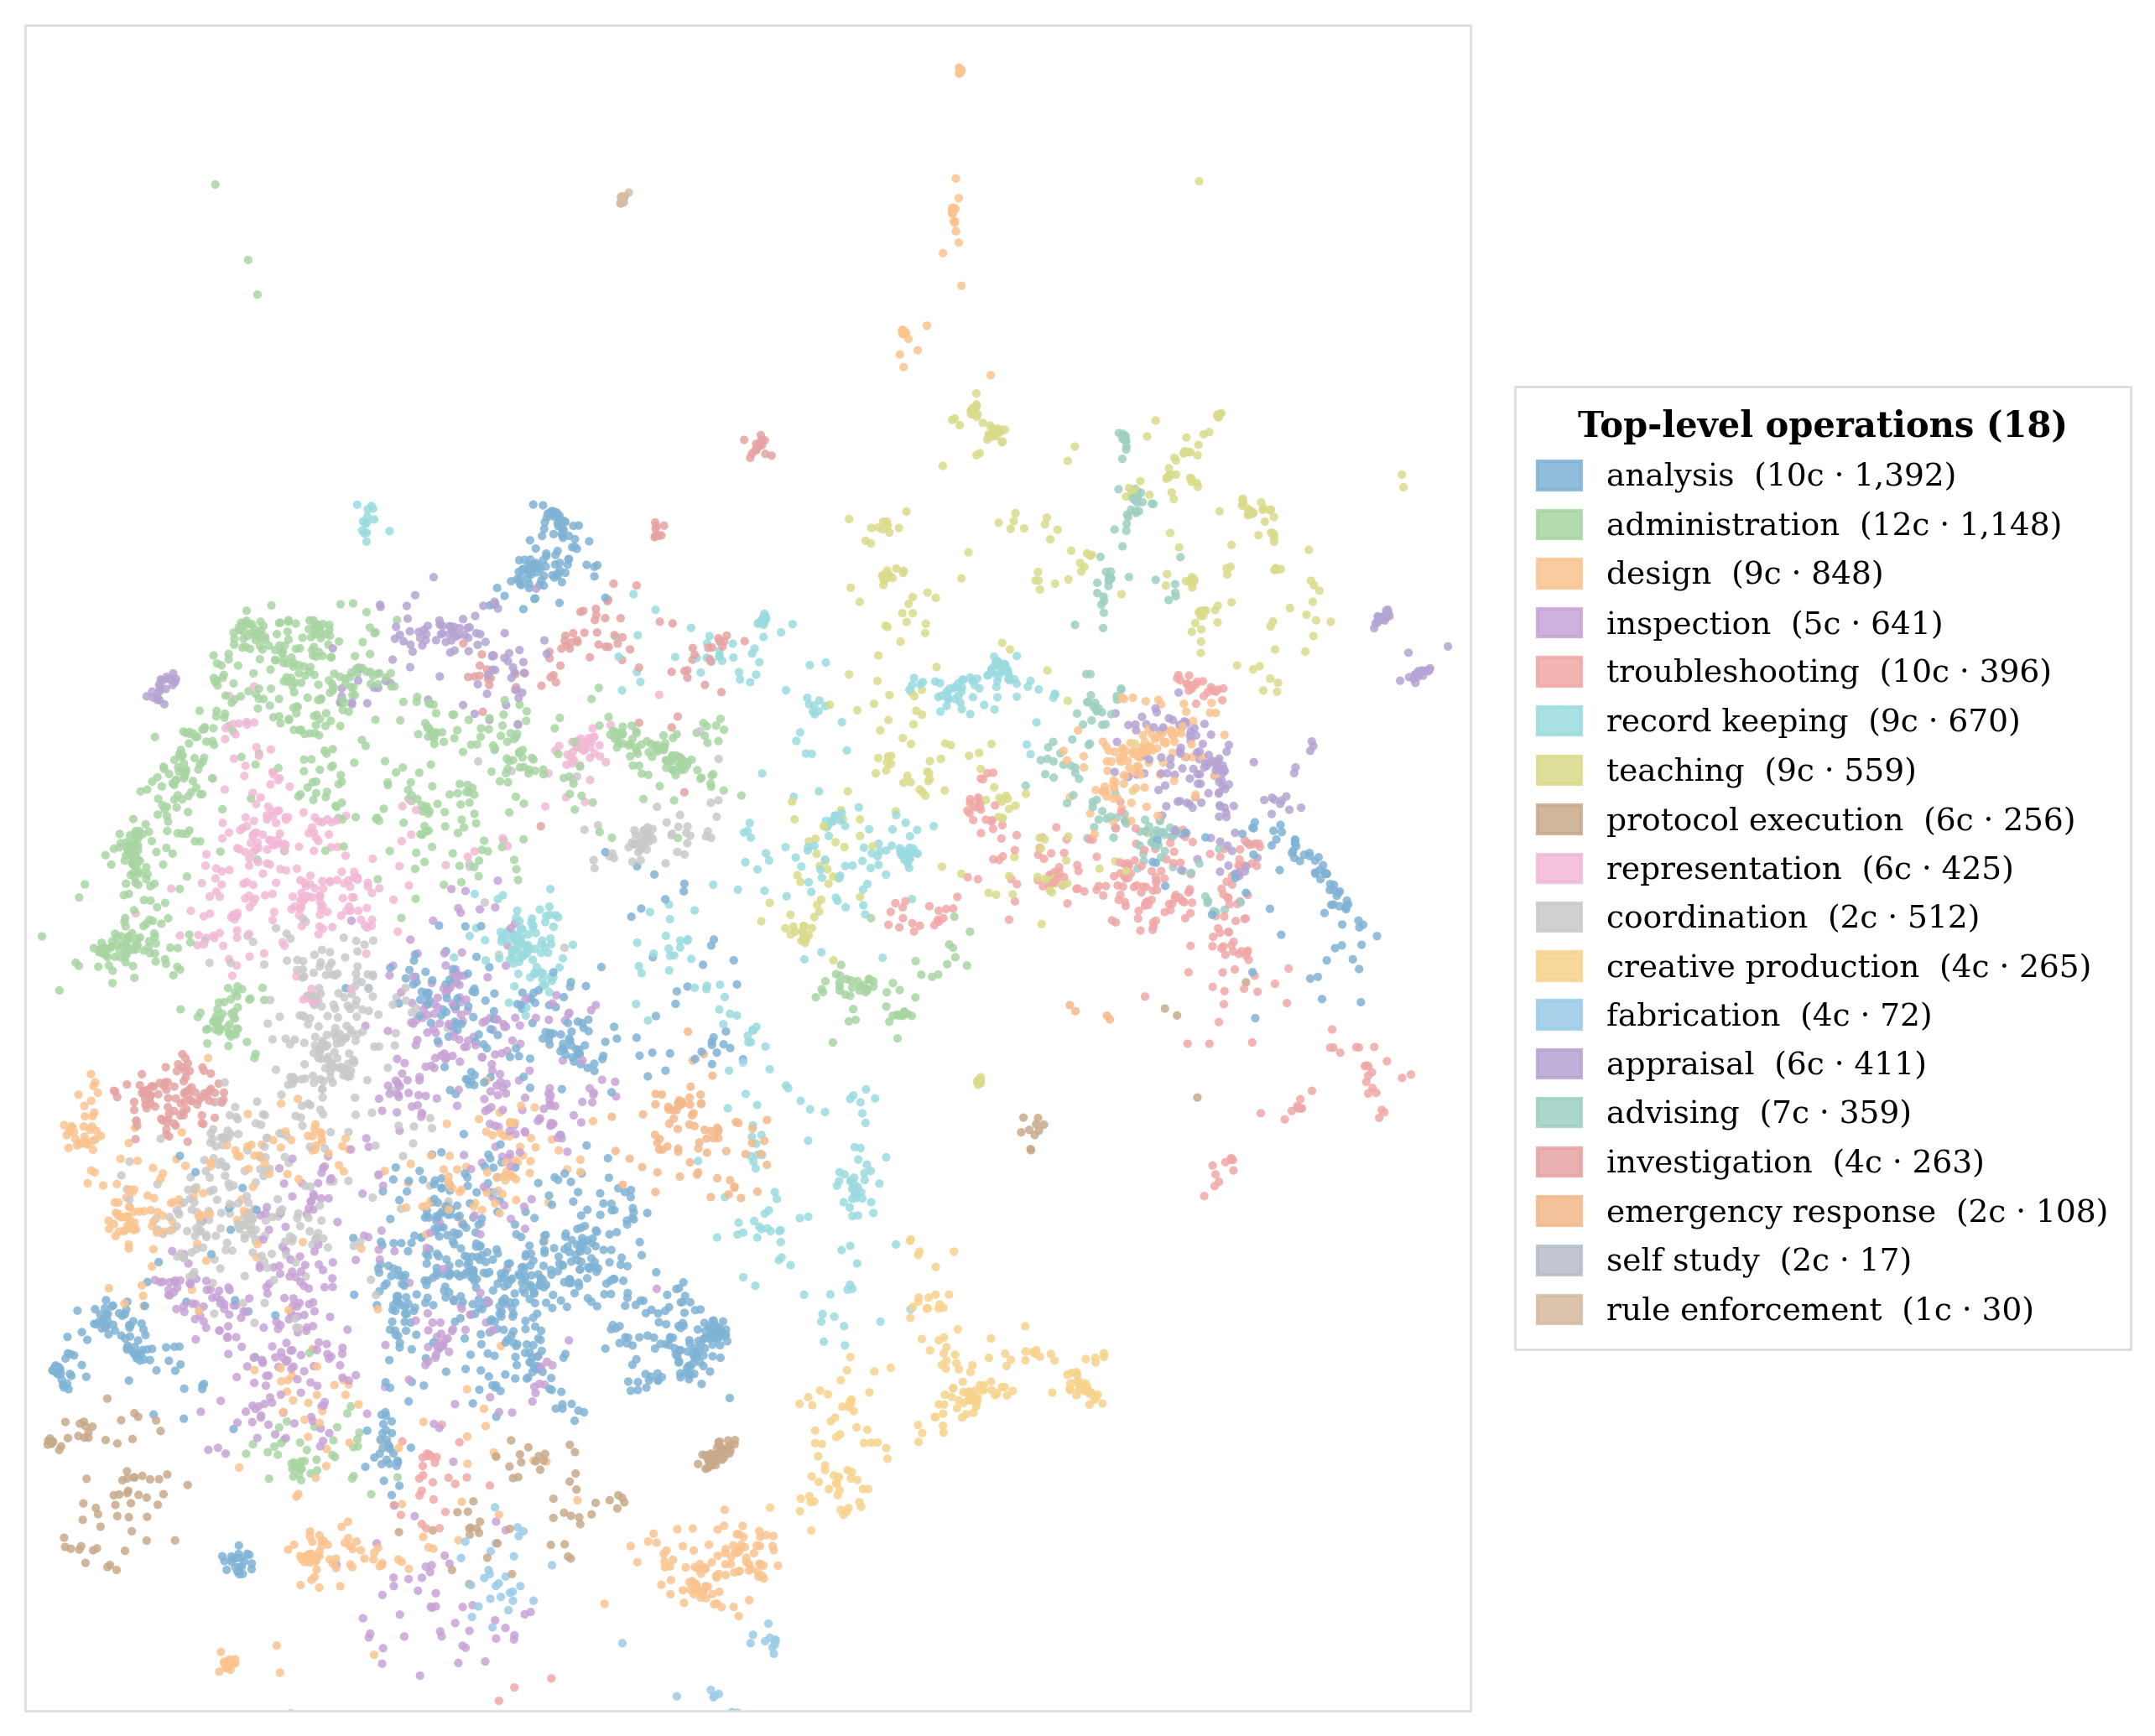
\includegraphics[width=0.82\linewidth]{operation_atlas.png}
\caption{Operation atlas of O{*}NET knowledge work.
The plot shows the 8{,}372 task statements retained after the stricter task-level screen, drawn from the 12{,}464-task Job-Zone-3--5 knowledge-work corpus.
The layout is a UMAP projection of 1{,}536-dimensional task embeddings; color denotes the final operation label.
The figure is a qualitative visualization of the operation space, not a quantitative measure of benchmark coverage or validity.
Pipeline details are in Appendix~\ref{app:taxonomy}.}
\label{fig:atlas}
\end{figure}

Figure~\ref{fig:atlas} plots retained tasks after domain-neutral paraphrase, density-based clustering, and expert consolidation (recipe: Appendix~\ref{app:taxonomy}; layout uses UMAP \citep{mcinnes2018umap} on embeddings whose 108 dense HDBSCAN groups \citep{campello2013density} precede panel merge).
Each point is one task; colour is the final operation (Table~\ref{tab:ops}).
UMAP preserves local neighbourhoods in the usual sense (similar normalised wording tends to sit nearby), but the two-dimensional layout is not a quantitative work-similarity map.
Colour-separated islands often reflect different surface vocabularies for the same underlying operation; the central band typically mixes labels where generic verbs (\emph{plan}, \emph{assess}, \emph{document}) pull disparate tasks together, and the codebook's distinct-from constraints disambiguate what geometry alone cannot.

Disconnected regions that share a colour mark cross-occupation structure: the same abstraction (e.g.\ evidence $\to$ findings) appears in different occupational contexts (laboratory analysis versus legal analysis), so a benchmark that samples only one region tests a fragment of the operation as the atlas defines it.
Embodied and protocol-heavy work (\emph{fabrication}, \emph{emergency-response}, parts of \emph{protocol-execution}) often appears as smaller or peripheral concentrations because the task-level screen removes tasks whose primary content is manual, performative, or routine-clerical rather than judgement on records.
Those regions are a reminder that ``knowledge work'' in the O{*}NET-derived sense still includes activities an LLM cannot complete without a body or a controlled environment; benchmark claims about ``professional'' assistance should not silently assume that only desk-and-language tasks exist in the reference set.

The figure does not validate any benchmark.
It shows the empirical variety the taxonomy compresses into eighteen labels and therefore sets a coverage target: cross-occupation evaluation should sample across the colour-specific regions that matter for the operation under test.

\paragraph{Observations.} Three features of Figure~\ref{fig:atlas} bear directly on the paper's argument beyond the reading rules above.
The largest operations (\emph{analysis}, \emph{administration}, \emph{troubleshooting}, \emph{inspection}, \emph{record-keeping}) are not single-occupation: they occupy multiple disjoint regions of the layout because their constituent tasks come from genuinely different occupations (quantitative analysis of laboratory data versus legal analysis of case law) yet share the same underlying abstraction (evidence $\to$ findings).
A substantial slice of the corpus is embodied: \emph{fabrication}, \emph{emergency-response}, \emph{rule-enforcement}, and parts of \emph{protocol-execution} shrink under the task-level screen because their tasks describe physical, performative, or direct-manual work.
These constitute the LLM-dark half of professional work, covering occupations of high economic weight whose outputs an LLM cannot produce on its own.
The dense centre of the atlas mixes logically distinct operations whose short-form vocabulary overlaps (plan, assess, document) even though their grading criteria differ.
Every operation therefore carries explicit distinct-from contrasts rather than relying on embedding geometry alone.

\section{Operation mapping tables}
\label{app:mapping}

The distinct-from and cross-occupation-examples fields carry most of the semantic weight of the taxonomy.
Distinct-from prevents adjacent operations from collapsing under short-form vocabulary (``\emph{plan}'', ``\emph{assess}'', ``\emph{document}''); cross-occupation examples enforce cross-occupation coverage.
Table~\ref{tab:distinctfrom} reproduces the pairwise contrasts and Table~\ref{tab:crossjob} reproduces the cross-occupation example sets directly from the taxonomy.

% --- auto-generated mapping tables ---
\begin{table}[p]
\caption{\emph{distinct-from} pairwise contrasts per operation. Each operation carries an explicit contrast against every adjacent operation whose embedding-space proximity risks collapse under short-form vocabulary (e.g.\ \emph{plan}, \emph{assess}, \emph{document}). These contrasts are invariants of the taxonomy: they are what allows a grading rubric for an operation to avoid silently scoring a different operation.}
\label{tab:distinctfrom}
\centering
\scriptsize
\begin{tabularx}{\linewidth}{l X}
\toprule
operation & \emph{distinct-from} contrasts \\
\midrule
\emph{analysis} & \emph{appraisal}: appraisal uses a pre-specified rubric to produce a score; analysis produces open-ended findings.; \emph{investigation}: investigation reconstructs a specific past event; analysis is broader interpretive work.; \emph{record-keeping}: record-keeping stores / retrieves existing records; analysis generates new findings from them.; \emph{design}: design specifies something new to build / deliver; analysis interprets what exists. \\
\emph{administration} & \emph{coordination}: coordination aligns people on specific projects; administration runs steady-state functions.; \emph{representation}: representation is external-facing; administration is internal org-running. \\
\emph{design} & \emph{fabrication}: fabrication physically builds the thing; design only specifies it.; \emph{analysis}: analysis is about existing evidence; design is about a new artefact. \\
\emph{inspection} & \emph{investigation}: investigation reconstructs a specific past event; inspection checks present compliance.; \emph{appraisal}: appraisal produces a score / value; inspection produces a compliance verdict.; \emph{troubleshooting}: troubleshooting fixes; inspection only reports. \\
\emph{troubleshooting} & \emph{protocol-execution}: protocol-execution follows a pre-scripted procedure with no diagnostic reasoning; troubleshooting requires figuring out what is wrong first.; \emph{inspection}: inspection only checks against rules; it does not fix.; \emph{emergency-response}: emergency-response is acute-crisis; troubleshooting is non-acute diagnose-and-fix. \\
\emph{record-keeping} & \emph{analysis}: analysis produces new findings from records; record-keeping stores and retrieves them.; \emph{creative-production}: creative-production makes original works; record-keeping maintains references.; \emph{administration}: administration runs HR / finance / ops as a process; record-keeping maintains documents. \\
\emph{teaching} & \emph{advising}: advising is personalized to one client's case; teaching delivers content that applies to the whole group / learner.; \emph{protocol-execution}: protocol-execution makes a principal productive; teaching makes a learner competent.; \emph{self-study}: self-study is the learner doing it themselves; teaching is the instructor side. \\
\emph{protocol-execution} & \emph{troubleshooting}: troubleshooting requires diagnosis; protocol-execution follows specified steps.; \emph{fabrication}: fabrication builds a new physical artefact; protocol-execution runs a specified process. \\
\emph{representation} & \emph{coordination}: coordination is internal alignment; representation is outward-facing.; \emph{advising}: advising is serving a client with personalized guidance; representation is soliciting / persuading external parties on behalf of the org. \\
\emph{coordination} & \emph{administration}: administration runs steady-state org machinery (HR / finance / ops); coordination is task / project-scoped alignment.; \emph{representation}: representation engages external audiences; coordination is internal. \\
\emph{creative-production} & \emph{fabrication}: fabrication makes utilitarian physical objects; creative-production makes creative / media works.; \emph{record-keeping}: record-keeping maintains existing records; creative-production generates originals. \\
\emph{fabrication} & \emph{design}: design only specifies on paper; fabrication produces the physical thing.; \emph{creative-production}: creative-production makes creative / media artefacts; fabrication makes utilitarian physical objects.; \emph{protocol-execution}: protocol-execution runs a process; fabrication creates a new physical artefact. \\
\emph{appraisal} & \emph{inspection}: inspection produces a pass/fail against rules; appraisal produces a score or value on a scale.; \emph{analysis}: analysis is open-ended interpretation of evidence; appraisal applies a pre-specified rubric.; \emph{investigation}: investigation reconstructs a past event; appraisal values / grades a current item. \\
\emph{advising} & \emph{teaching}: teaching delivers general content to a group/learner; advising is 1:1 and tailored to one case.; \emph{analysis}: analysis produces findings from evidence; advising produces a recommendation for an individual.; \emph{representation}: representation engages external audiences for a transaction/commitment; advising is client-serving. \\
\emph{investigation} & \emph{inspection}: inspection is a present-state compliance check; investigation is a retrospective reconstruction.; \emph{analysis}: analysis is broader interpretive work; investigation targets a specific past event / wrongdoing. \\
\emph{emergency-response} & \emph{troubleshooting}: troubleshooting is non-acute diagnose-and-fix; emergency-response is acute crisis stabilization.; \emph{rule-enforcement}: rule-enforcement is ongoing behavioral control; emergency-response is acute. \\
\emph{self-study} & \emph{teaching}: teaching makes others learn; self-study is the practitioner learning themselves.; \emph{analysis}: analysis produces new findings as a deliverable; self-study builds personal competency. \\
\emph{rule-enforcement} & \emph{emergency-response}: emergency-response is acute-crisis; rule-enforcement is ongoing.; \emph{inspection}: inspection audits things / processes; rule-enforcement governs people. \\
\bottomrule
\end{tabularx}
\end{table}

\begin{table}[p]
\caption{\emph{cross-occupation-examples} per operation. The cross-profession invariant requires that every top-level operation carries examples from at least three distinct professional families. Examples are literal quotes from the final taxonomy JSON (\emph{data/derived/manual\_labeling/operation\_taxonomy.json}).}
\label{tab:crossjob}
\centering
\scriptsize
\begin{tabularx}{\linewidth}{l X}
\toprule
operation & cross-job examples \\
\midrule
\emph{analysis} & scientists and postsecondary researchers; policy analysts and economists; lawyers, judges, judicial clerks; data analysts / scientists / bioinformaticians; GIS analysts and surveyors; radiologists / pathologists interpreting instrumental output; environmental and climate analysts \\
\emph{administration} & department heads and general managers; HR / labor relations / compensation / benefits; supervisors, foremen, production managers; purchasing / logistics / supply-chain analysts; budget analysts, controllers, accountants, auditors; loan officers, credit analysts, bookkeepers \\
\emph{design} & curriculum / instructional designers; treatment and case-management planners; mechanical / electrical / civil / controls engineers; software and database architects; urban planners and architects; solution architects and product designers \\
\emph{inspection} & safety, environmental, building, and code inspectors; QA / QC and software QA; calibration and telecom test technicians; hazmat / biosafety compliance officers; regulatory compliance auditors \\
\emph{troubleshooting} & auto, diesel, and industrial mechanics; IT incident responders and network engineers; HVAC / wind-turbine / power-plant troubleshooters; physicians, nurses, NPs, PAs in assess-and-treat; PT / OT / speech / behavioral therapists; veterinarians; dental / audiology / optometry / prosthetics; cosmetologists and aestheticians \\
\emph{record-keeping} & administrative and clerical staff; medical-records and clinical admin; social workers / case managers documenting cases; librarians, archivists, historians; editors, proofreaders, technical writers; translators and medical interpreters \\
\emph{teaching} & classroom and postsecondary teachers; corporate trainers; clergy preaching; coaches and fitness / rehab instructors; clinical educators; safety and compliance trainers \\
\emph{protocol-execution} & lab technicians (bio / chem / materials / forensic / clinical); sterility and infection control across lab, surgical, dental, food; aviation pilots, flight engineers, ATC; ship captains, marine engineers; power-plant / hydro / process-plant operators; surgical techs and nursing assistants; medical / dental / vet assistants; legal assistants and paralegals; research and laboratory assistants; engineering technicians and drafters; teaching aides \\
\emph{representation} & executives, legislators, clergy representing institutions; sales account managers and negotiators; PR, development, fundraising; supply-chain / procurement negotiators; marketing campaign leads \\
\emph{coordination} & project and program managers; executive assistants and event planners; research coordinators; engineers and clinicians conferring cross-functionally \\
\emph{creative-production} & musicians, composers, choreographers, dancers; graphic / game / set designers and fine artists; photographers, camera operators, desktop publishers; producers, directors, journalists, broadcast and film editors \\
\emph{fabrication} & jewelers, machinists, patternmakers, craft artists; plumbers, electricians, HVAC and solar installers; telecom and motor repairers; aircraft and industrial maintenance mechanics \\
\emph{appraisal} & teachers grading work; HR / performance appraisers; clinical evaluators (psych, OT, PT); real-estate and damage appraisers; claims adjusters and eligibility workers; peer reviewers and certifiers \\
\emph{advising} & financial advisors; physicians / NPs in consultation; career and school counselors; management consultants; clergy pastoral counseling; mental-health and rehab counselors; sales engineers doing site-assessment proposals \\
\emph{investigation} & police, detectives, fraud examiners; intelligence and security analysts; forensic pathologists, coroners; insurance / IG investigators; cybersecurity forensics \\
\emph{emergency-response} & firefighters, police, EMS, paramedics; ER physicians and nurses; disaster management and utility incident response; air-traffic controllers in incident response \\
\emph{self-study} & every regulated / licensed profession — medicine, law, accounting, engineering, teaching, nursing, therapy, finance \\
\emph{rule-enforcement} & teachers and coaches enforcing classroom rules; corrections and security officers; airline / transit crew enforcing safety rules; compliance officers enforcing conduct policies \\
\bottomrule
\end{tabularx}
\end{table}

\section{External-taxonomy legibility: ESCO}
\label{app:esco}

This appendix contains the full experiment referenced from Section~\ref{sec:realwork}: scope, design, pipeline, per-operation coverage and shares, and a reading of the cases where the O{*}NET and ESCO per-operation distributions diverge.

\paragraph{Source and scope.} The ESCO inputs are the v1.1.1 English CSV release \citep{esco2022v111}, ingesting the Skills pillar, the Occupations pillar (with the ISCO groups table), and the occupation--skill relations.
The scope filter keeps rows whose skill type is skill or competence and retains only skills that are essential-linked to at least one occupation in ISCO-08 groups 1, 2, or 3, giving 5{,}826 items.
A supplementary set of 1{,}977 knowledge-type items is excluded from the primary analysis because such ESCO rows describe subject-matter domains rather than work operations.

\paragraph{Design.} O{*}NET remains the derivation dataset and the taxonomy is held frozen.
Pooling is avoided on construct grounds: ESCO's primary unit is the \emph{skill / competence}, whose text is a description of an ability a worker must hold, while O{*}NET tasks are descriptions of work performed.
The two units sit at different construct levels, and mixing them in a single clustering run would blur the primary claim.
The scope filter (skill or competence type, essential-linked to at least one ISCO-08 group 1-3 occupation~\citep{ilo2012isco08}) is the ESCO analogue of the O{*}NET Job Zones 3--5 scope.
The resulting 5{,}826 items are assigned to one of the 18 operations by an LLM prompted with the frozen per-operation one-line definition, input, output, and distinct-from fields, plus an explicit ``none of the above'' option for items the taxonomy does not cover.
The two signals we report are mapping coverage under this rubric assignment and the per-operation distribution of ESCO items against the O{*}NET distribution from Section~\ref{sec:realwork}.
The divergences localise the places where the taxonomy is most O{*}NET-shaped, and their direction is interpretable from how the two ontologies are built.

\paragraph{LLM assignment.} An LLM classifier is called once per item at temperature 0 with a system prompt that contains the 18 operation ids and, for each, the one-line definition, input, output, and up to three distinct-from clauses.
The prompt requires the model to return an operation id, a confidence rating of high, medium, or low, and a one-sentence rationale, and explicitly permits a ``none of the above'' label for items that do not describe a work operation.
Classification calls are cached so the pass is resumable.
Of the 5{,}826 scoped items, 3{,}893 return high confidence (66.8\%), 1{,}642 medium (28.2\%), and 291 low (5.0\%).
A supplementary centroid assignment (cosine similarity of each ESCO item to the $L_{2}$-normalized mean of O{*}NET task embeddings per operation) is computed for cross-reference but is not used for any number reported in this appendix.

\paragraph{Mapping coverage.} 5{,}730 of the 5{,}826 ESCO items (98.3\%) are placed into one of the 18 operations; 96 items (1.7\%) receive a ``none of the above'' label.
All 18 operations receive ESCO items; 17 of 18 receive $\geq\!40$ items, with \emph{investigation} the single exception at 39.
The ``none of the above'' set is dominated by ESCO entries that encode personal traits (``exercise patience'', ``tolerate stress'', ``have emotional intelligence''), subject-matter knowledge (``types of tile'', ``energetic meridians''), perceptual abilities (``differentiate nuances of colour''), or language-proficiency labels (``speak different languages''), all of which describe attributes rather than operations and whose rejection is consistent with the taxonomy's operation-not-worker design rule.
The atlas therefore absorbs the ESCO material at the categorical level: no operation empties, no large residue accumulates outside the taxonomy.
Where the two corpora diverge is in how they re-weight the 18 operations, which we read next.

\paragraph{Where O{*}NET and ESCO diverge.} Figure~\ref{fig:esco_share} and Table~\ref{tab:esco_coverage} give the per-operation shares in each corpus.
Every operation is populated in both, but the two corpora re-weight the 18 categories substantially.
The re-weighting is not random; it tracks a construction-level difference between the two ontologies.
O{*}NET is a per-occupation task inventory: each occupation in the database receives roughly 25 imperative task statements written by occupational analysts, and the corpus accumulates statements across professions, so activities every profession must document separately (filing, logging, reporting, maintaining) multiply as new professions are added.
ESCO is a skill-competence catalogue derived from EU qualification frameworks: each ESCO item is written once at a competence level and linked to many occupations, and the competence unit privileges transferable capabilities (coordinating, advising, designing) over discrete stewardship acts.
The two ontologies therefore occupy overlapping semantic space at different granularities.
Where O{*}NET multiplies, ESCO aggregates; where ESCO multiplies, O{*}NET aggregates.

O{*}NET's over-weight relative to ESCO (O{*}NET percent minus ESCO percent, in operation-share percentage points) is concentrated on discrete stewardship acts.
\emph{troubleshooting} ($+5.1$pp) reflects the many maintenance, diagnosis, and repair task statements O{*}NET writes for JZ 3--5 technical occupations (technicians, maintenance engineers, IT support, equipment operators), where ESCO collapses the same work into a smaller number of broader technical-problem-solving competences.
\emph{administration} ($+4.5$pp) and \emph{record-keeping} ($+1.9$pp) are the same mechanism applied to clerical overhead: O{*}NET names filing, scheduling, documenting, and reporting as standalone tasks for nearly every professional occupation, while ESCO rarely codes documentation as a competence distinct from the broader professional skill it supports.
\emph{investigation} ($+2.3$pp) and \emph{appraisal} ($+1.6$pp) reflect O{*}NET's habit of writing profession-specific investigative and review tasks (for auditors, detectives, researchers; for credit officers, appraisers, compliance officers) where ESCO recodes the same work under analytical or inspection-type competences.
\emph{teaching} ($+2.1$pp) reflects O{*}NET splitting pedagogy into explain / demonstrate / evaluate tasks per instructor occupation while ESCO codes pedagogy as one or two transferable competences.
\emph{analysis} ($+2.0$pp) is smaller than the others because analysis is named at the competence level in both ontologies, but O{*}NET still records many profession-specific analytical tasks on top.

ESCO's over-weight relative to O{*}NET is concentrated on transferable competences.
\emph{advising} ($+5.6$pp) and \emph{fabrication} ($+5.4$pp) are the two largest gaps.
Advising is over-weighted in ESCO because the ontology carries an unusually rich vocabulary of advice-giving as a named transferable competence across consultants, counsellors, and client-facing advisors, whereas O{*}NET distributes the same work across ``explain to client,'' ``review with client,'' and ``make recommendations'' task strings that scatter into adjacent operations.
Fabrication is over-weighted because ESCO carries many named craft-skill and technical-execution competences for ISCO group 3 Technicians (specific assembly, installation, operating, and processing procedures) that survive the knowledge-work scope filter; on the O{*}NET side, many analogous tasks were removed earlier by the direct-embodied screen.
\emph{coordination} ($+3.8$pp) reflects ESCO naming cross-functional and temporal coordination as a standalone competence required for most ISCO 1-3 roles, where O{*}NET embeds coordination inside composite task statements.
\emph{design} ($+3.6$pp) reflects ESCO's coverage of engineering, architecture, and creative qualifications producing many named design competences, where O{*}NET splits the underlying activity into analyse / specify / draft / review tasks.
\emph{rule-enforcement} ($+2.0$pp) is the starkest case of O{*}NET undersampling: O{*}NET contains only 30 tasks in this operation (Table~\ref{tab:ops}) because it scopes rule-enforcement work to the few occupations whose primary function is enforcement (police, inspectors), while ESCO has a rich compliance, conduct, and ethics vocabulary linked as \emph{essential} to many regulated professions.

A single generalisation covers most of the pattern.
Where O{*}NET names many small profession-bound tasks for one underlying activity, ESCO names one broad profession-abstract competence for the same activity; where ESCO splits a broad competence into several named subcompetences, O{*}NET lumps them under a single named task.
The 18-operation taxonomy sits at a granularity closer to O{*}NET's task level, so the taxonomy's per-op counts under-represent the activities ESCO multiplies (advising, fabrication, coordination, design, rule-enforcement) and over-represent the activities O{*}NET multiplies (troubleshooting, administration, record-keeping, investigation, teaching).
The divergence is a statement about the unit of analysis, not about whether the operations themselves are real: the same operations appear under both ontologies and absorb items in both, only at different shares.

\paragraph{Reading.} The atlas remains largely legible under ESCO: 98.3\% of scoped items are placed, every operation is populated, and the ``none of the above'' residue is small and concentrated on non-operation items.
The point of the study is not that ESCO \emph{confirms} the 18 operations; it did not see the taxonomy during derivation, and its unit of analysis is different.
The point is that the taxonomy carries enough structure across ontologies to be read against ESCO material, and that the places where the two corpora disagree are informative.
The distribution comparison flags the O{*}NET-shaped regions of the atlas: small-$n$ O{*}NET operations (\emph{rule-enforcement} at 30 tasks), operations whose O{*}NET phrasing has no direct ESCO analogue (\emph{investigation}, \emph{appraisal}), and the U.S./EU re-weighting across \emph{troubleshooting}, \emph{administration}, \emph{record-keeping}, \emph{advising}, \emph{fabrication}, \emph{coordination}, and \emph{design}.
A taxonomy derived on ESCO material would probably carve these regions differently, and the research programme the paper argues for would benefit from rebuilding the atlas on a multi-ontology base when the resources allow.

\begin{figure}[t]
\centering
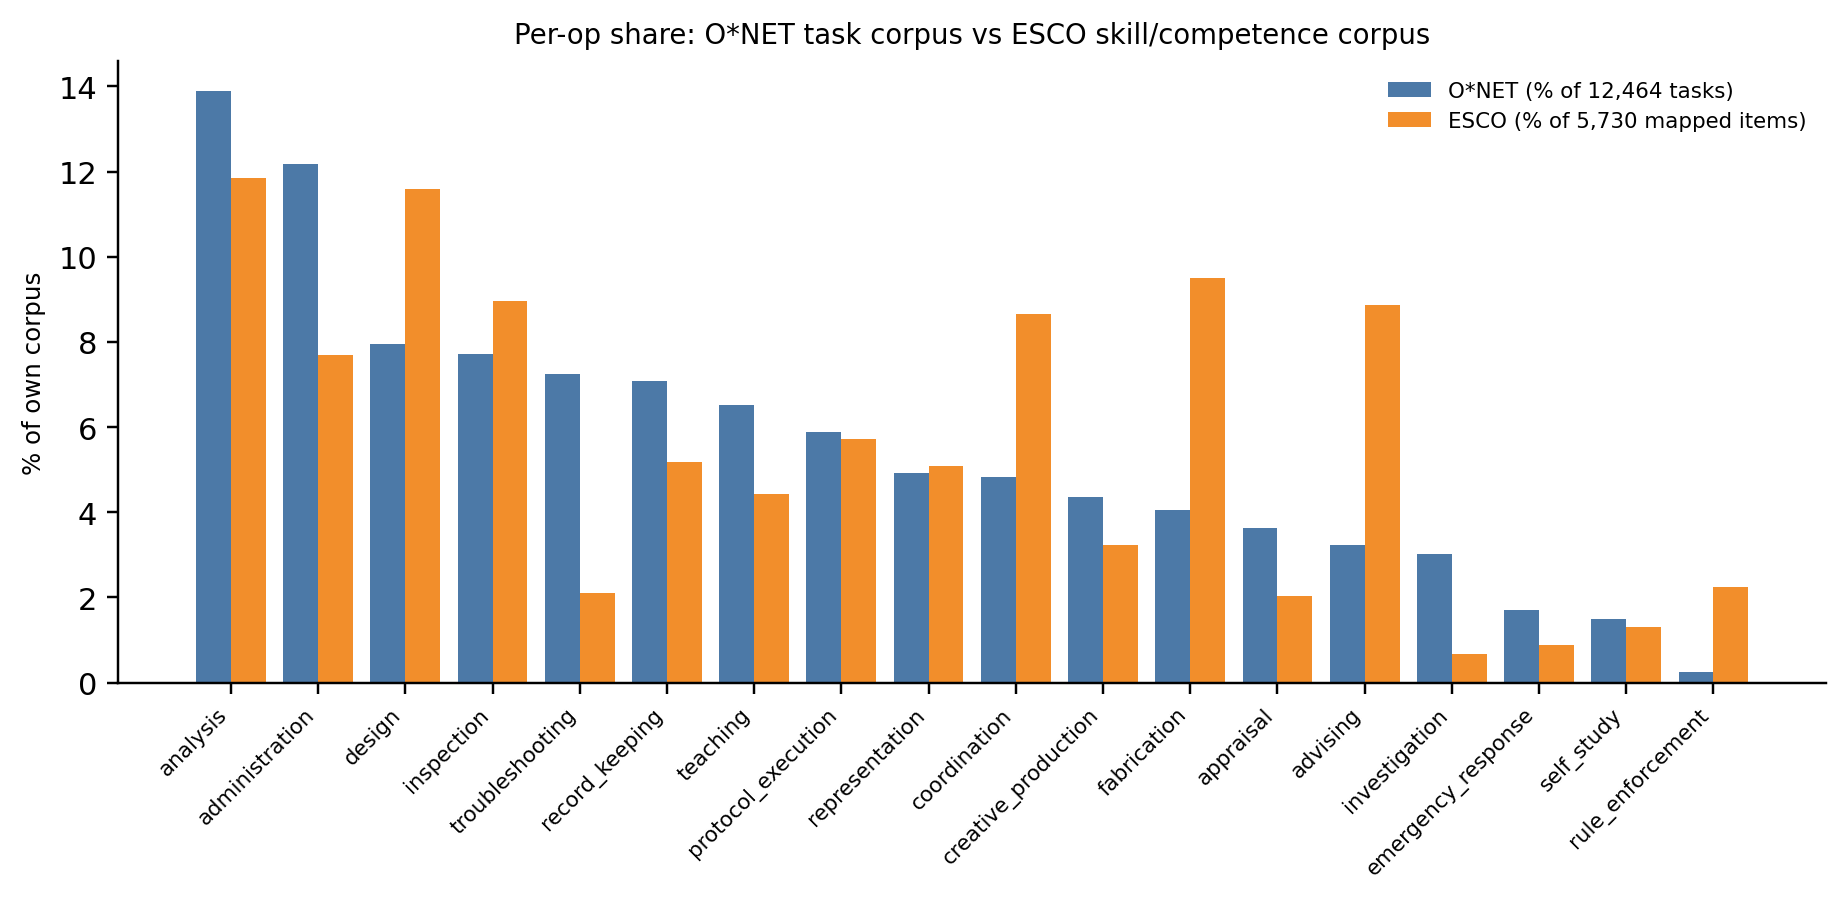
\includegraphics[width=0.98\linewidth]{esco_onet_op_share.png}
\caption{\textbf{Per-operation share in the O{*}NET task corpus
  (12{,}464 knowledge-work tasks) versus the scoped ESCO
  skill/competence corpus (5{,}730 items mapped to an operation).}
  Both corpora populate all 18 operations. The two catalogues
  re-weight the operations substantially: ESCO emphasises
  \emph{advising}, \emph{fabrication}, \emph{coordination},
  \emph{design}, and \emph{rule-enforcement} more than O{*}NET;
  O{*}NET emphasises \emph{troubleshooting}, \emph{administration},
  \emph{record-keeping}, \emph{investigation}, and
  \emph{teaching} more than ESCO. The direction of the divergence
  tracks the two ontologies' different units of analysis
  (profession-bound tasks vs profession-abstract competences), as
  read in Appendix~\ref{app:esco}. Underlying counts are in
  Table~\ref{tab:esco_coverage}.}
\label{fig:esco_share}
\end{figure}

\begin{table}[t]
\caption{Per-operation shares in the O{*}NET task corpus versus the
  scoped ESCO skill/competence corpus. \textbf{O{*}NET $n$} is the
  task count from Table~\ref{tab:ops}. \textbf{ESCO $n$} is the number
  of scoped ESCO items assigned to the operation by the LLM
  classifier. \textbf{$\Delta$} is ESCO percent minus
  O{*}NET percent in operation-share percentage points. Sorted by
  $\Delta$.}
\label{tab:esco_coverage}
\centering
\footnotesize
\begin{tabular}{lrrrrr}
\toprule
operation & O{*}NET $n$ & O{*}NET \%\ & ESCO $n$ & ESCO \%\ & $\Delta$ (pp) \\
\midrule
\emph{troubleshooting}      &    902 &  7.2 & 120 &  2.1 & $-5.1$ \\
\emph{administration}       & 1{,}517 & 12.2 & 441 &  7.7 & $-4.5$ \\
\emph{investigation}        &    377 &  3.0 &  39 &  0.7 & $-2.3$ \\
\emph{teaching}             &    814 &  6.5 & 254 &  4.4 & $-2.1$ \\
\emph{analysis}             & 1{,}732 & 13.9 & 679 & 11.9 & $-2.0$ \\
\emph{record-keeping}      &    882 &  7.1 & 297 &  5.2 & $-1.9$ \\
\emph{appraisal}            &    453 &  3.6 & 116 &  2.0 & $-1.6$ \\
\emph{creative-production} &    543 &  4.4 & 185 &  3.2 & $-1.1$ \\
\emph{emergency-response}  &    212 &  1.7 &  50 &  0.9 & $-0.8$ \\
\emph{self-study}          &    186 &  1.5 &  75 &  1.3 & $-0.2$ \\
\emph{protocol-execution}  &    735 &  5.9 & 328 &  5.7 & $-0.2$ \\
\emph{representation}       &    615 &  4.9 & 292 &  5.1 & $+0.2$ \\
\emph{inspection}           &    963 &  7.7 & 514 &  9.0 & $+1.2$ \\
\emph{rule-enforcement}    &     30 &  0.2 & 128 &  2.2 & $+2.0$ \\
\emph{design}               &    992 &  8.0 & 664 & 11.6 & $+3.6$ \\
\emph{coordination}         &    603 &  4.8 & 496 &  8.7 & $+3.8$ \\
\emph{fabrication}          &    505 &  4.1 & 544 &  9.5 & $+5.4$ \\
\emph{advising}             &    403 &  3.2 & 508 &  8.9 & $+5.6$ \\
\midrule
\textbf{total}                & \textbf{12{,}464} & \textbf{100.0} & \textbf{5{,}730} & \textbf{100.0} & \\
\bottomrule
\end{tabular}
\end{table}

\section{Precedents for the two-layer structure}
\label{app:precedents}

Section~\ref{sec:two-layers} cites the canonical sources for the separation of score meaning and score use \citep{messick1989validity,jacobs2021measurement}, the separation of artefact specification from situated functioning \citep{suchman1987plans}, and the separation of technical capability from organisational complements \citep{bresnahan2002it}.
This appendix records the recent empirical work that registers the same cut in workplace settings, and that motivates pairing task validity with organisational validity rather than collapsing them.

AI assistance produces gains on some knowledge tasks for consultants and losses on others, with the boundary difficult for users to anticipate \citep{dellacqua2023jagged}.
A field deployment of a generative-AI tool for customer support shows task-level productivity gains distributed unevenly across workers, with novices gaining most and experienced workers gaining little \citep{brynjolfsson2023genai}.
Microsoft Research's \emph{Generative AI in Real-World Workplaces} report \citep{microsoft2024workplaces} and related CHI work \citep{tankelevitch2024metacognitive} document that realised workplace effects depend strongly on how users and organisations integrate the tools into existing practice.
These literatures each render one side of the cut the present account requires on both sides simultaneously, leaving the two layers not reducible to each other.

\section{Benchmark audit: case material}
\label{app:benchcases}

This appendix reports per-suite case material that grounds the verdicts of Section~\ref{sec:whybench} in concrete task and rubric examples.
Counts are computed from the released task and rubric files; example text is quoted directly.
Table~\ref{tab:audit-three} consolidates the three audited suites' verdicts against the framework's two axes; the per-suite paragraphs that follow ground each cell in the relevant task, rubric, and reward-spec evidence.

\begin{table}[!htbp]
\caption{Audit verdicts on the three audited suites against the framework's two axes (Section~\ref{sec:whybench}). Task validity decomposes into grounding (G), boundedness (B), and handoff (H); organizational validity decomposes into authority (A), accountability (Ac), and integration (I).}
\label{tab:audit-three}
\centering
\scriptsize
\setlength{\tabcolsep}{4pt}
\renewcommand{\arraystretch}{1.15}
\begin{tabular}{p{0.10\linewidth} p{0.27\linewidth} p{0.31\linewidth} p{0.22\linewidth}}
\toprule
suite & coverage & task validity (G / B / H) & organizational validity (A / Ac / I) \\
\midrule
\textsc{GDPval} & 220 tasks across 44 occupations sampled in nine sectors; one-shot deliverable shells of \emph{analysis}, \emph{design}, \emph{record-keeping}, \emph{advising}, \emph{creative-production}, \emph{inspection}; judgment-in-acquisition removed by the prompt designer (43.2\% of tasks supply zero reference files; median 1) & ${\approx}91\%$ of items reward artifact form (mechanical 4.8\%, institutional 6.6\%, other 80.2\%); substantive items (8.3\%) are closed-form named-correctness statements; boundedness implicit; handoff unscored & not tested: authority, accountability, integration absent from criterion set \\
\addlinespace[2pt]
$\tau^2$-Bench & 2{,}546 episodes across four customer-service domains (89.7\% telecom); partial \emph{administration}, \emph{coordination}, \emph{troubleshooting}; O{*}NET Job Zone~2 (vocational), distinct from the framework's Job Zone 3--5 anchor & strongest of three on grounding and boundedness; user pre-loaded with problem, persona, and acceptance criteria, removing the interpretive layer; within-episode handoff scored & not tested: simulator terminates at episode end; no ticket queue, account-note system, escalation owner, or filing path \\
\addlinespace[2pt]
\textsc{APEX-Agents} & 480 tasks across investment banking, consulting, corporate law; 33 worlds (22 fully fictional, 9 real-companies-in-fictional, 2 mixed); 87.9\% inline reply; \emph{record-keeping}, \emph{protocol-execution}, \emph{appraisal}, \emph{creative-production} excluded by reply-only output shape & closest current public match to the framework's definition of knowledge work: in-world files, disabled web search, structured prompts; and yet the supporting workspace is authored for the benchmark, prompts pre-supply analytical scaffolding, the rubric vocabulary punishes premise interrogation, and the artifactual surface is ignored on 87.9\% of tasks & not tested: roleplay engagements; no real partner, client, filing path, or downstream consumer of the agent's output \\
\bottomrule
\end{tabular}
\end{table}

\paragraph{\textsc{GDPval}: rubric depth on a small per-occupation sample.}
\textsc{GDPval} releases five tasks per occupation in 44 occupations.
A representative task for the \emph{Accountants and Auditors} occupation asks the agent to author an Excel workbook supporting an audit-sample selection: compute a sample size at 90\% confidence and 10\% tolerable error, perform quarter-on-quarter variance analysis, and select the audit sample under named criteria (e.g., $>20\%$ variance, specific entities and divisions).
The task carries 47 rubric criteria spanning four kinds.
\emph{Mechanical} criteria check delivery format (``The submitted deliverable is an Excel workbook file whose basename is `Sample'\ldots'').
\emph{Substantive} criteria check named correctness statements (``The `Sample Size Calculation' worksheet uses a standard attribute sampling formula with $z=1.645$, $p=0.5$, $e=0.10$, and applies finite population correction'').
\emph{Institutional} criteria check fidelity to reference materials (``For every row included on the first worksheet, the values in columns A--H exactly match the corresponding row in the Population reference'').
\emph{Other} criteria check task-specific content presence (``The first tab contains at least one sample where the division is Corporate Banking, the sub-division is Corporate Loans, and the country is Italy'').
The rubric carries explicit penalties for output-fidelity violations, including $-10$ for delivering a lossy audio format and $-20$ when an audio deliverable contains a description of the mixing process but no audio drawn from the reference set.
The set of operations exercised across tasks is heterogeneous: this Accountants task is a hybrid \emph{record-keeping} and \emph{analysis} bundle; tasks in \emph{Audio and Video Technicians} are \emph{creative-production}; tasks in \emph{Compliance Officers} are \emph{inspection}.
The score is therefore a per-deliverable signal computed against a high-density rubric, with the rubric tailored to the task rather than to the represented operation.

\paragraph{$\tau^2$-Bench: programmatic checks on a stateful customer-service episode.}
A representative $\tau^2$-Bench-Telecom task simulates a roaming customer abroad whose mobile data is failing and who will only accept ``excellent'' speed.
The agent and the simulated user share access to phone-status tools (toggling roaming, checking message capability, reading the status bar) and a programmatic environment.
The reward specification names two environment assertions the world must satisfy at episode end (mobile data is enabled and the reported internet speed equals ``excellent'') and one expected user-side action (toggling roaming).
The Boolean reward fires only when the environment assertions hold; the action-trace check is a soft signal.
Substantively, the agent must follow a troubleshooting tree under telecom-specific policy.
The episode terminates inside the simulator: there is no test of whether the customer's plan, ticket, or escalation queue is updated in any system the operator would actually consult after the call.
The score is therefore a within-episode coordination signal.

\paragraph{\textsc{APEX-Agents}: short binary criteria on a file-rich workspace.}
A representative \textsc{APEX-Agents}-Law task supplies a Master Supply Agreement and asks whether a supplier may invoke force majeure after a U.S. tariff change.
The agent works inside a world that contains 161 files on average (documents, PDFs, email, chat, spreadsheets) with web search disabled.
The grading rubric for this task contains three binary criteria, each phrased as a positive statement the response must contain: ``States Yes, the supplier can invoke the force majeure clause under the terms of the Master Supply Agreement'', ``States that the force majeure clause can be invoked for tariff increases of more than 25\%'', and ``States that goods from Iraq are subject to a 35\% tariff per Trump's July 20, 2025 announcement''.
The expected output is a chat reply, not a memo or filed document.
This shape is dominant in the suite: 422 of 480 tasks expect an inline message, while only 58 (12.1\%) expect a created or edited artifact such as a new document, spreadsheet, or slide deck.
The score is therefore a fact-presence signal computed inside an authentic professional-services workspace.

\paragraph{What the cases together show.}
The three suites differ in scored unit (deliverable, episode, message), in rubric design (high-density human rubric, programmatic reward spec, short binary criterion list), and in environment fidelity (closed task with reference files, stateful simulator, multi-application world).
They share the limit that no scored unit reaches the organizational layer.
\textsc{GDPval} grades a deliverable; $\tau^2$-Bench grades an interaction inside a closed simulator; \textsc{APEX-Agents} grades a reply inside a workspace that resembles a professional engagement.
Authority, accountability, sign-off, record integration, and downstream review are not part of the reward in any of the three.
This is the source of the claim limitation in Section~\ref{sec:rollup}.

\section{Full strict-coverage audit table}
\label{app:audit-table}

Table~\ref{tab:audit} extends the per-suite reasoning of Section~\ref{sec:whybench} to a wider sample of public benchmarks.
\textbf{Strict cover} requires (1)~full op, not primitive; (2)~$\geq 3$ profession families within the scored scope; (3)~realistic artefact output; (4)~realistic input horizon; (5)~op-relevant grading.
Under this rubric no benchmark in the sample strictly covers any operation.
Verdicts are \textbf{primitive-only} (a sub-primitive of the operation), \textbf{partial / single-domain} (the operation in one profession), \textbf{partial / primitive} (the operation in puzzle-shaped form), \textbf{partial / cross-profession} (the operation across several professions, with grading still short of the institutional layer), or \textbf{absent} (no operation targeted).
Entries should be read as claims about the benchmark's scope, not about the capability of any model that runs on it.

\begin{table}[!htbp]
\caption{Strict coverage verdicts for public LLM and agent
  benchmarks against the 18-operation taxonomy.}
\label{tab:audit}
\centering
\scriptsize
\setlength{\tabcolsep}{4pt}
\renewcommand{\arraystretch}{1.1}
\begin{tabular}{p{0.21\linewidth} p{0.18\linewidth} p{0.16\linewidth} p{0.40\linewidth}}
\toprule
benchmark (scored unit) & nearest op & verdict & principal gap \\
\midrule
\multicolumn{4}{l}{\textit{Question-answering and recall.}} \\
MMLU                                & \emph{self-study} / \emph{analysis} & primitive-only & multiple-choice recall + one-step reasoning; neither the practitioner-current output nor the open-ended interpretation is produced. \\
ARC, HellaSwag, TriviaQA            & \emph{self-study}                & primitive-only & knowledge / commonsense recall; no learning-process measured. \\
SQuAD, NaturalQuestions, BoolQ      & \emph{record-keeping}            & primitive-only & single-passage extractive QA; covers one sub-step of the retrieve-curate-translate-serve loop. \\
KILT, BEIR retrieval suites         & \emph{record-keeping}            & primitive-only & corpus-level retrieval; misses translation, curation, cross-format maintenance. \\
TruthfulQA, HaluEval                & cross-cutting                       & primitive-only & faithfulness / hallucination is a cross-cutting property of op outputs, not an op. \\
Winograd, WSC, SuperGLUE            & none                                & primitive-only & linguistic primitives. \\
\addlinespace[2pt]
\multicolumn{4}{l}{\textit{Reasoning and verification.}} \\
GSM8K, MATH, AIME, MMLU-STEM        & \emph{analysis}                   & primitive-only & arithmetic / mathematical reasoning; a primitive inside \emph{analysis}, \emph{appraisal}, and \emph{inspection}. \\
FEVER, FacTool, AVeriTeC            & \emph{investigation}              & primitive-only & single-claim verification; \emph{investigation} requires reconstructing past events from distributed evidence. \\
CNN/DM, XSum, MultiNews             & \emph{analysis}                   & primitive-only & single-source summarisation, ROUGE-graded; no synthesis across evidence, no expert grading. \\
HELM-instruct, InstructEval         & mixed                               & primitive-only & broad instruction-following; each scenario is an op fragment, no scenario tests an operation end-to-end. \\
\addlinespace[2pt]
\multicolumn{4}{l}{\textit{Domain-bound analysis and inspection.}} \\
LegalBench: issue-spotting          & \emph{analysis} (primitive)       & primitive-only         & multiple-choice issue labels; not the memo artefact. \\
LegalBench: rule-application        & \emph{analysis} / \emph{inspection} & partial / primitive & IRAC steps; profession-bound; short-answer grading. \\
LegalBench: rhetorical              & \emph{analysis} (primitive)       & primitive-only         & classification of legal rhetoric; not an op output. \\
LegalBench: contract review         & \emph{inspection}                 & partial / single-domain & compliance checks against rules; output shape matches \emph{inspection}; one profession. \\
ContractNLI, CUAD                   & \emph{inspection}                 & partial / single-domain & clause classification / extraction; one sub-step of \emph{inspection} in one domain. \\
FinanceBench                        & \emph{analysis}                   & partial / single-domain & financial-filings QA; realistic inputs, one profession. \\
FinQA, TAT-QA                       & \emph{analysis} (financial)       & partial / single-domain & tabular-plus-text numeric analysis; domain-bound. \\
BioASQ, PubMedQA                    & \emph{analysis} (biomedical)      & partial / single-domain & biomedical evidence to finding; domain-bound. \\
\addlinespace[2pt]
\multicolumn{4}{l}{\textit{Code generation and software engineering.}} \\
HumanEval, MBPP, APPS               & \emph{design}                     & partial / single-domain & function-level specification; software engineers only. \\
BigCodeBench, LiveCodeBench         & \emph{design}                     & partial / single-domain & larger / fresher corpora; same single-profession bar. \\
ClassEval                           & \emph{design}                     & partial / single-domain & class-level code generation; software engineers only. \\
SWE-bench, SWE-Lancer               & \emph{troubleshooting}            & partial / single-domain & cleanest existing instance of \emph{troubleshooting}; software-only. \\
\addlinespace[2pt]
\multicolumn{4}{l}{\textit{Agent and workflow benchmarks.}} \\
GAIA                                & \emph{analysis} + \emph{record-keeping} & partial / primitive & heterogeneous but puzzle-shaped; short final answers, not the report / record artefact. \\
BrowseComp                          & \emph{record-keeping} $\to$ \emph{analysis} & primitive-only & web-retrieval puzzle; no deliverable. \\
AgentBench: SQL / filesystem / cards & various                            & primitive-only         & tool use and planning in constrained environments; no operation end-to-end. \\
AgentBench, Mind2Web, WebArena, VisualWebArena & \emph{coordination} / \emph{administration} & partial / single-domain & web-agent tasks; consumer web / developer tools only. \\
WorkArena                           & \emph{administration}             & partial / single-domain & ServiceNow only; single enterprise stack. \\
OSWorld                             & \emph{administration} / \emph{troubleshooting} & partial / primitive & OS-task completion; short episode. \\
OfficeBench                         & \emph{administration}             & partial / primitive     & Office-app task completion; single-doc scope. \\
AssistantBench                      & \emph{administration}             & primitive-only          & consumer-web assistant tasks; not safety-critical procedure execution. \\
\addlinespace[2pt]
\multicolumn{4}{l}{\textit{Clinical, creative, and dialogue.}} \\
AgentClinic, MedQA clinical vignettes & \emph{troubleshooting} (diagnostic) + \emph{advising} & partial / single-domain & diagnose-then-recommend in one profession; cross-job condition fails. \\
MedQA rote, USMLE step exams        & \emph{self-study}                & primitive-only          & recall of clinical knowledge; the maintenance-of-competency operation is not measured. \\
\textsc{HealthBench-Professional}~\citep{arora2025healthbench}   & \emph{advising} (clinical)        & partial / single-domain & physician-written closed-form rubric over single-turn case responses; pre-supplied case description; no chart note, order entry, referral, or audit-trail object on which the response can be filed or reviewed. \\
MedAgentBench                       & \emph{administration} + \emph{protocol-execution} & partial / single-domain & FHIR-resource scoring; medicine only. \\
Reddit WritingPrompts, CREATIVE-WRIT & \emph{creative-production}      & partial / single-domain & one medium scored; visual design, photo / video, edited media not covered. \\
MusicCaps, AudioCaps                & \emph{creative-production} (criticism) & primitive-only    & captioning, not producing the artefact. \\
CICERO, Diplomacy, Rampage          & \emph{representation}             & partial / single-domain & negotiation in game settings; no real-stakes external engagement. \\
LMSYS Chatbot Arena                 & none                                & absent                  & pairwise preference on free-form chat; not graded on operation criteria. \\
\addlinespace[2pt]
\multicolumn{4}{l}{\textit{Audited in detail in Section~\ref{sec:whybench}.}} \\
\textsc{GDPval}                     & 44 occupations sampled              & partial / corpus-level  & blind expert preference; per-task scoring fails the $\geq\!3$-profession condition; institutional layer untested. \\
$\tau^2$-Bench                      & \emph{administration} + \emph{coordination} & partial / single-domain & policy-derived ground truth; one domain (customer service); handoff terminates inside the simulator. \\
\textsc{APEX-Agents}                & \emph{analysis} + \emph{advising} & partial / cross-profession & data-rich worlds across three professional-services jobs; rubric grading; no sign-off, filing, or liability. \\
\bottomrule
\end{tabular}
\end{table}

\section{Per-benchmark coverage reasoning}
\label{app:perbench}

This appendix expands Section~\ref{sec:whybench}, stating the coverage verdict for each benchmark family by shape.

\paragraph{Single-profession analysis suites.} \textsc{LegalBench}~\citep{legalbench2023} and \textsc{FinanceBench}~\citep{financebench2023} are the highest-fidelity QA-shaped suites in the sample.
Their inputs are realistic (case documents, SEC filings); their authors have explicit task decompositions; and they are essential as operationalisations of \emph{legal reasoning} and \emph{financial QA}.
They do not, however, satisfy the cross-occupation requirement, nor do they instantiate the deliverable-bundle shape: LegalBench items are short-answer or multiple-choice at the scored-unit level, and FinanceBench items are closed-book QA rather than memo authorship.
Reading a strong score as a ``legal-analysis capability'' or ``financial-analysis capability'' overclaims the unit.

\paragraph{General-purpose web and desktop agents.} \textsc{BrowseComp}~\citep{browsecomp2024}, \textsc{GAIA}~\citep{gaia2023}, and \textsc{OSWorld}~\citep{osworld2024} target a wide input surface but grade short, puzzle-shaped outputs.
They are correctly read as \emph{primitive} scores (retrieval competency, tool use, web navigation) rather than operation scores.
Their environments are realistic; their \emph{episodes} are not: the task typically terminates at a short string, not at a stateful artefact that survives into review.

\paragraph{Stateful enterprise agents.} \textsc{WebArena}~\citep{webarena2023} and \textsc{WorkArena}~\citep{workarena2024} are the closest the public sample gets to realistic \emph{administration}: stateful environments, multi-step episodes, action-grounded scoring.
\textsc{OfficeBench}~\citep{officebench2024} adds office-document automation.
All three pay for this realism with single-stack scope (ServiceNow, consumer web, Office), which prevents satisfaction of the three-profession criterion.
They are, by our rubric, \emph{partial / single-domain} covers and the most promising base on which an operation-shaped \emph{administration} benchmark could be built.

\paragraph{Clinical agents.} \textsc{MedAgentBench}~\citep{medagentbench2024} scores structured clinical workflow tasks against an EHR: placing IV catheters, setting up ventilators, and administering medications.
It is distinctively good on \emph{fidelity}: the scored artefacts are produced FHIR resources with strict equivalence checks rather than natural language, and so it clears the op-relevant-grading criterion, covering both clinical \emph{administration} and the clinical slice of \emph{protocol-execution}.
Its scope is, by construction, one profession.

\paragraph{Software engineering.} The SWE lineage is the audited sample's only operation-shaped family.
\textsc{SWE-bench}~\citep{jimenez2024swebench} made agentic real-repo evaluation credible; its extensions \textsc{APEX-SWE}~\citep{kottamasu2026apex} and \textsc{SWE-bench Pro}~\citep{swebenchpro2025} push difficulty toward integration, operations, and multi-language reality; and code-review suites \citep{sweprbench2025,codefusecrbench2025,withmartiancr2024} target \emph{appraisal} rather than authorship.
Collectively they score \emph{troubleshooting} and \emph{design} on real repositories with professional grading (tests + rubric + reviewer comments).
What they do not do is span occupations: they are the existence proof that the rubric is tractable, not its instantiation at scale.

\section{Five failure surfaces}
\label{app:surfaces}

This appendix expands Section~\ref{sec:rollup} by stating the five recurring mechanisms that separate public benchmarks from the operations they are read as measuring.

The \emph{benchmark dataset} is typically either profession-narrow (\textsc{SWE-bench}, \textsc{LegalBench}, \textsc{MedQA}) or heterogeneous but puzzle-shaped (\textsc{GAIA}, \textsc{BrowseComp}); both shapes fail to sample the cross-occupation structure Figure~\ref{fig:atlas} makes visible.
The \emph{benchmark rubric} is dominated by exact-match, ROUGE/BLEU, or pairwise preference, whereas real operations are graded professionally on coverage, faithfulness, auditability, fitness-for-purpose, and the absence of named institutional failure modes.
The \emph{benchmark task} is scored at the model-turn level, not at the deliverable-bundle level; episodes that require review, sign-off, or hand-off are truncated at ``model said something.''
The \emph{benchmark environment} is usually stateless and single-actor, whereas real operations run in stateful worlds (files, inboxes, tickets, versions, CRMs, EHRs) where the integration \emph{is} in carrying state; agent environments (\textsc{WorkArena}, \textsc{OSWorld}, \textsc{MedAgentBench}) are honest exceptions, and remain single-profession.
\emph{Benchmark failure analysis} collapses into a single scalar (accuracy, pass@k, reward), whereas real operations have institutional failure modes (wrongful deletion, lost version, right-answer-wrong-authority, missed reviewer, unauditable edit) that do not show up in aggregate accuracy.
Without a failure-mode taxonomy the scalar cannot rule out costly failures.

\section{Unit of analysis and structural features}
\label{app:unit-features}

This appendix elaborates the operation as the unit of analysis, referenced in Section~\ref{sec:realwork}.

\paragraph{Why the operation is the unit.} Two alternative units of analysis are natural, and both fail under inspection.
One is the \emph{primitive} (retrieve, extract, classify, reason, answer, patch).
Primitives are attractive because cheap verifiers exist for them and they compose, but a professional deliverable is not a superposition of primitive correct answers; it is graded on coverage, faithfulness, fitness-for-purpose, auditability, and the absence of named institutional failure modes, and these criteria are not visible from primitive success rates.
Scoring the primitive and licensing an operation-level claim is the category error Section~\ref{sec:rollup} names.
The second alternative is the \emph{occupation} (or \emph{profession}): evaluate legal work, financial work, or clinical work as irreducible suites, the route taken by much of the economics-of-AI literature.
Occupation-indexed suites support exposure estimation but cannot, by construction, distinguish a model that generalises a work pattern across occupations from a model narrowly trained on one occupation's vocabulary, which is precisely the distinction that bears on whether a capability claim generalises outside its training domain.
The \emph{operation} is the smallest unit that simultaneously (i)~carries a recognisable professional construct (diagnose, appraise, execute a protocol, synthesise evidence into findings) that practitioners can grade, (ii)~recurs in more than one occupation so that a benchmark built on it is cross-occupation by construction, and (iii)~is small enough to be instantiated in a bounded sandbox.
These three criteria, not the word itself, are what the rest of the paper leans on.

\paragraph{Why $\geq\!3$ profession families.} The same criteria motivate the $\geq\!3$-profession-family clause of the strict-cover rule.
\emph{One} profession is vacuously satisfiable by any suite built within a single domain (\textsc{LegalBench}, \textsc{FinanceBench}, \textsc{SWE-bench}).
\emph{Two} is consistent with a shared vocabulary or a shared regulatory origin: accounting and auditing, radiology and pathology, and several medical sub-specialties are pairwise close enough that a two-profession instantiation can be absorbed by a single domain model without ever exercising the cross-occupation generalisation the operation names.
\emph{Three} distinct families force the benchmark to instantiate the operation under genuinely different input surfaces, review chains, and failure modes; it is the smallest number at which the ``single-domain artefact'' reading can be ruled out on the face of the data.
The threshold is also the one we respect when deriving the taxonomy itself: every operation in Table~\ref{tab:ops} carries $\geq\!3$ distinct profession families in its cross-occupation example invariant.
Relaxing the threshold to two would admit covers that collapse under a single domain model; strengthening it to four would disqualify operations whose professional instantiation is genuinely narrow (\emph{emergency-response}, \emph{rule-enforcement}) without changing which benchmarks clear the bar.

\paragraph{Structural features evaluation must preserve.} Table~\ref{tab:features} names the features a benchmark must preserve to measure the operation rather than a primitive inside it.
Each row is a property the operation already has in professional practice and that a benchmark must instantiate if it is to license an operation-level claim.

\begin{table}[t]
\caption{Structural features of professional work versus what
  standard benchmarks usually instantiate.}
\label{tab:features}
\centering
\footnotesize
\begin{tabularx}{\linewidth}{lXX}
\toprule
feature & real professional work & typical benchmark \\
\midrule
output shape  & deliverable bundle (doc + memo + email + spreadsheet version) & single string / short answer \\
state         & mutation of canonical state (doc, DB, ticket) under permissions & string grader; state not modelled \\
context       & raw, versioned evidence; authority and permissions matter & pre-digested snippet; authority implicit \\
episode       & continues through review, sign-off, audit, next actor & ends at ``model said something'' \\
grading       & expert rubric / review lane / failure-mode taxonomy & exact match, ROUGE/BLEU, pairwise preference \\
traceability  & provenance: source, version, authority, timestamp, reviewer & unrecorded \\
\bottomrule
\end{tabularx}
\end{table}

\section{Detailed responses to alternative views}
\label{app:altviews}

This appendix expands Section~\ref{sec:altviews} with the full responses to each counterargument.

One counterargument to our position is that benchmarks target task fragments because fragments scale.
They are easier to sample, often profession-agnostic, and can be checked with exact match, unit tests, or other cheap verifiers.
The objection has weight because scalable measurement is one reason AI research made progress on coding benchmarks.
It supports using primitive scores as diagnostic signals.
It does not support citing those scores as operation-level capability claims.
A retrieval benchmark can show that a model finds information; it cannot show that a model produced a research memo that is grounded, within scope, reviewable, and usable by the next actor.
The adoption~/~capability overhang \citep{a16z2026adoption,brynjolfsson2026playbook} is partly what happens when a diagnostic signal is treated as a work claim.

Another counterargument attributes the overhang to security, integration, change-management, and data-access frictions.
This objection is also strong.
Real deployments fail for many reasons that benchmarks cannot solve.
The point is that these frictions become harder to reason about when the underlying capability claim is unclear.
If a benchmark never tests permissions, review handoff, or state changes in the receiving system, it cannot separate model capability from deployment risk.
Better operation-shaped evaluation would leave many deployment problems in place, yet it would make the remaining problems interpretable.

Expert grading at scale is expensive and slow, which is the central practical challenge for the position.
We do not ask every benchmark to become a manual expert panel; we point instead to verifier-side infrastructure: simulators, human-rubric lanes, reusable failure-mode taxonomies, and public corpora of real work.
Code-review benchmarks \citep{sweprbench2025,codefusecrbench2025,withmartiancr2024} show how one operation (\emph{appraisal}~/~\emph{inspection}) can become cheaper when the field has a public work corpus and checkable review criteria.
The open question is which other operations can support similar verification paths.

\section{Operations under the lens of AI agents}
\label{app:opslens}

For each of the 18 operations, Table~\ref{tab:opslens} names the main AI-task translation and the principal open problem standing between naming an operation and scoring it.
The table is a research-agenda map.
Almost every operation's open problem calls for realistic stakes, stateful environments, expert-calibrated grading, and a named failure-mode taxonomy: the same features Table~\ref{tab:features} lists as constitutive of professional work.
Building any one of these instruments well is plausibly a multi-year research programme, and none of the eighteen has been built end-to-end, cross-occupation, at credible fidelity.

\begin{table}[t]
\caption{Operations under the lens of AI agents: one-line AI-task
  translation and principal open problem, per operation.}
\label{tab:opslens}
\centering
\scriptsize
\begin{tabularx}{\linewidth}{lXX}
\toprule
operation & AI-task translation & principal open problem \\
\midrule
\emph{analysis} & open-ended interpretive memo from a heterogeneous evidence pile, graded by expert rubric on coverage + faithfulness + novelty. & sourcing expert-graded memos at scale; rubric agreement across professions. \\
\emph{administration} & multi-platform workflow agent against stateful enterprise record systems (ServiceNow + Workday + SAP + EHR) with auditable change logs. & cross-platform sandboxes; permission~/~authority model; policy-compliance scoring. \\
\emph{design} & produce a spec that downstream actors can execute end-to-end, cross-domain beyond software (process, service, organisation). & non-software ground truth; ``does the spec produce a working artefact?'' validators outside unit tests. \\
\emph{inspection} & multi-clause review of a submitted artefact against stated rules, producing a cited findings document across $\geq\!3$ regulated professions. & rubric agreement across professions; citation-level grading; adversarial clause variation. \\
\emph{troubleshooting} & diagnose-then-fix loop outside SWE: mechanical-repair simulators, clinical differential~+~treatment, IT incident response, HVAC. & sandbox fidelity; ground-truth fix validation that isn't unit-test pass. \\
\emph{record-keeping} & multi-format record-maintenance agent: retrieve + curate + translate + serve with provenance. & version-control reasoning; cross-format consistency; retention-policy compliance as a scoreable property. \\
\emph{teaching} & evaluation scored on \emph{learner outcome}, not model Q\&A accuracy: does the learner's competency demonstrably rise after the session? & longitudinal learner-level ground truth; ethical constraints on randomised teaching arms. \\
\emph{protocol-execution} & agent executing a prescribed procedure end-to-end across domains (clinical orders, flight pre-check, emergency SOP) graded on deviation class. & realistic protocol sandboxes; deviation taxonomy; acceptance-criteria calibration with domain experts. \\
\emph{representation} & multi-turn external engagement with real-stakes output (contract clause closed, settlement, disclosure filed) scored on outcome \emph{and} process. & adversarial counterparty simulation; stakes fidelity; grading process without incentivising theatre. \\
\emph{coordination} & multi-agent orchestration across roles (lead + reviewers + approvers) with auditable hand-offs across tools and time. & ground truth for ``coordination went well'' that isn't reducible to atomic task success. \\
\emph{creative-production} & multi-medium delivered artefact (text + image + video + edit) adjudicated by calibrated expert panels. & reproducible creative grading; anti-gaming; cost of expert adjudication. \\
\emph{fabrication} & instruction-following in a simulated or supervised physical environment, or expert review of work plans~/~build documentation. & embodied-verification bridge; most of \emph{fabrication} sits outside an LLM's reach without instrumented environments. \\
\emph{appraisal} & LLM-as-judge on \emph{real} submissions (code review, contract review, peer review, grading) calibrated against expert rubrics. & anti-gaming; reviewer-bias audit; multi-reviewer calibration; stability under adversarial submissions. \\
\emph{advising} & extended advising session with longitudinal client state, scored on decision quality and regret. & synthetic clients that drift realistically; stake fidelity; regret estimation without the actual outcome. \\
\emph{investigation} & multi-source evidence reconstruction producing a case narrative with attribution, scored on evidence coverage, attribution correctness, false-positive rate. & ground-truth case corpora with adversarial evidence placement. \\
\emph{emergency-response} & time-pressured tool-using agent in a simulated emergency (dispatch triage, medical code, cyber incident) graded on containment, escalation appropriateness, time-to-action. & simulator fidelity; outcome ground truth; grading escalation without over-incentivising escalation. \\
\emph{self-study} & longitudinal evaluation: does the model~/~practitioner stay current with a drifting field over time? & defining ``current'' reproducibly; scoring a trajectory; avoiding knowledge-cutoff contamination. \\
\emph{rule-enforcement} & contextual moderation~/~compliance enforcement with escalation judgement, scored on fairness, consistency, escalation-appropriateness across adversarial cases. & adversarial test-set design; fairness-audit methodology; policy-vs-contextual-exception reconciliation. \\
\bottomrule
\end{tabularx}
\end{table}

\end{document}
